% ============================================================================
%  PHY 420 capstone thesis (full document)
%  Compile:  latexmk -pdf main.tex        (or just press Recompile in Overleaf)
%
%  Each section lives in sections/. intro_methods.tex builds the Introduction,
%  Theory and Methods alone for the partial submission, from the same files.
% ============================================================================
\documentclass[11pt,letterpaper]{article}
% ============================================================================
%  Shared preamble: packages and notation for main.tex and every partial build
%  (intro_methods.tex). One file, so a notation change is one edit.
% ============================================================================
\usepackage[margin=1in]{geometry}
\usepackage[T1]{fontenc}
\usepackage{lmodern}
\usepackage{microtype}
\usepackage{amsmath,amssymb,bm}
\usepackage{graphicx}
\usepackage{flafter}   % a float never appears before the text that introduces it
\usepackage{booktabs}
\usepackage{siunitx}
\usepackage{xcolor}
\usepackage{tikz}
\usetikzlibrary{positioning, arrows.meta, calc}
\usepackage[numbers,sort&compress]{natbib}
% The bibliography style is apsrev4-2. It reads its switches (article titles on)
% from a control entry in refs.bib that must be cited before anything else. That
% entry produces no reference, so natbib is told the key exists.
\makeatletter
\AtBeginDocument{\@namedef{b@apsrev42Control}{}\nocite{apsrev42Control}}
\makeatother
\usepackage{caption}
\captionsetup{font=small,labelfont=bf}
\usepackage[colorlinks=true,allcolors=blue!60!black]{hyperref}

% Figures live one directory up, already exported as vector PDF by the scripts.
\graphicspath{{../figures/}}

% Operators used throughout, so a convention change is one edit.
\newcommand{\Zop}[1]{\hat{Z}_{#1}}
\newcommand{\Xop}[1]{\hat{X}_{#1}}
\newcommand{\Yop}[1]{\hat{Y}_{#1}}
\newcommand{\sigp}[1]{\hat{\sigma}^{+}_{#1}}
\newcommand{\sigm}[1]{\hat{\sigma}^{-}_{#1}}
\newcommand{\Lop}[1]{\hat{L}_{#1}}
\newcommand{\Hop}{\hat{H}}
\newcommand{\todo}[1]{\textcolor{red}{\textbf{[TODO: #1]}}}

\newcommand{\fullthesis}{}  % lets the shared Introduction outline Results and Discussion

\begin{document}

% Title page, contents, abstract: the order the PHY 420 thesis guidelines list.
\begin{titlepage}
  \centering
  \vspace*{1.6in}
  {\LARGE\bfseries A quantified error budget for quantum simulation\\[4pt]
   of the lattice Schwinger model\par}
  \vspace{0.6in}
  {\large Abror Niyazmetov\par}
  \vspace{0.35in}
  Senior thesis, Physics 420\\
  Department of Physics, Gettysburg College\\[10pt]
  Advisor: Dr.\ Kurt Andresen\par
  \vfill
  {\today\par}
  \vspace*{0.4in}
\end{titlepage}

\tableofcontents
\newpage

\begin{abstract}
Quantum computers can follow gauge theories in real time, where lattice Monte
Carlo fails, but each result carries Trotter error from discrete time steps,
shot noise from finitely many measurements, and hardware error. This thesis
separates the three for the lattice Schwinger model, quantum electrodynamics in
one dimension, on four sites and four simulated qubits, checking every stage
against exact diagonalisation. At 1000 shots the Trotter error on the particle
density falls below the shot noise at a step of 0.18 at $t = 3$. At that shot
count the pair-production signal is lost once the two-qubit gate infidelity
times the number of CX gates reaches about two at all three step sizes tried,
and the best step grows with the gate error. The violation of charge
conservation, measured without the exact answer, predicts that threshold with
an optimistic bias of 10 to 17\,\% for depolarising noise and a larger one for
dephasing on the gates, and misses it entirely for dephasing between time
steps, the noise model fitted to the first experiment on this system. A
sample-based Krylov method reaches a mean relative energy error of $10^{-3}$
with 12 shots per circuit, or 15 with gate error.
\end{abstract}
\newpage

% ============================================================================
\section{Introduction}
\label{sec:intro}
% ============================================================================

Gauge theories describe three of the four known forces of nature. The gauge
theory of quarks and gluons, quantum chromodynamics (QCD), cannot be solved by
expanding in a small coupling at the energies where protons and neutrons form.
Its predictions there come from lattice gauge theory: space and time are
replaced by a finite grid of points~\cite{wilson1974}, the theory becomes a very
large but finite statistical problem, and that problem is solved by Monte Carlo
sampling~\cite{creutz1980}. The approach now computes hadron masses and other
static properties from first principles~\cite{durr2008}, but it cannot follow
what happens in time.

Monte Carlo lattice calculations work
in imaginary, or Euclidean, time, where the weight of each field configuration
is a positive number and can be treated as a probability. Continuing to real
time turns those weights into complex phases. Contributions of opposite sign
cancel, the average becomes a small difference of large numbers, and the
statistical error grows exponentially with the simulated time and the size of
the system. This is the sign problem. Fermions bring a sign problem of their own
even in imaginary time, for example at nonzero density, and Troyer and Wiese
showed that a general solution to it is almost certainly out of reach, because
such a solution would solve every problem in the complexity class NP in
polynomial time~\cite{troyer2005}. Processes that need real time, such as the
breaking of the flux string between separating charges~\cite{hebenstreit2013},
particle production in strong fields, and the approach to equilibrium after a
heavy-ion collision, therefore remain largely out of reach of first-principles
calculation~\cite{banuls2020,bauer2023}.

A quantum computer does not have this problem. Feynman argued that a quantum
system can be simulated efficiently only by another quantum
system~\cite{feynman1982}. Lloyd made the argument constructive: a sequence of
quantum gates approximates the time-evolution operator $e^{-i\Hop t}$ of any
Hamiltonian built from local terms, with an error that can be made as small as
desired by shortening the time step~\cite{lloyd1996}. Jordan, Lee and Preskill
later gave quantum algorithms for scattering in an interacting quantum field
theory~\cite{jordan2012}. A quantum processor applies $e^{-i\Hop t}$ directly
and never forms the complex weights that defeat Monte Carlo sampling. For
real-time gauge dynamics, then, the case for quantum simulation rests on a
concrete physical argument~\cite{georgescu2014,dalmonte2016}.

\subsection{The Schwinger model as a test bed}

The usual first target is the Schwinger model, quantum electrodynamics (QED) in
one space and one time dimension~\cite{schwinger1962}. It is the simplest gauge
theory that shares the features of QCD that matter here. Its charges are
confined: on a line the electric field between two opposite charges has nowhere
to spread, so the energy stored between them grows linearly with their
separation~\cite{coleman1975}. When the stored energy exceeds the cost of a new
particle--antiparticle pair, the vacuum produces one and the flux string breaks.
The model also breaks chiral symmetry and has a vacuum angle
$\theta$~\cite{coleman1976}. Schwinger solved the massless case exactly. Its
spectrum is a single free particle of mass $g/\sqrt{\pi}$, where $g$ is the
charge, which can be read either as a photon that has acquired a mass or as a
tightly bound particle--antiparticle pair~\cite{schwinger1962}. The Hamiltonian
lattice formulation of Kogut and Susskind~\cite{kogut1975,banks1976} has since
been studied with strong-coupling series~\cite{hamer1997}, the density matrix
renormalisation group~\cite{byrnes2002} and matrix product
states~\cite{banuls2013}. A system with this many independent answers is a good
place to test a method.

Quantum simulations of the lattice Schwinger model now span a decade. After
proposals for trapped ions and cold atoms~\cite{banerjee2012,hauke2013},
Martinez \emph{et al.}\ carried out the first digital quantum simulation of a
lattice gauge theory in 2016, on four trapped-ion qubits~\cite{martinez2016}.
They eliminated the electric field by solving Gauss's law, so that four lattice
sites needed only four qubits, and they watched electron--positron pairs appear
out of the bare vacuum, the lattice state with no particles and no electric
field, over evolutions of more than 200 gates. Klco
\emph{et al.}\ simulated one and two spatial sites, that is two and four
staggered sites with periodic boundaries, on IBM superconducting processors,
keeping the electric field as explicit qubits with a cutoff and reducing their
number with symmetry projections~\cite{klco2018}. Kokail \emph{et al.}\
prepared ground states variationally on up to 20 qubits and estimated their own
error from the measured variance of the energy, without reference to a known
answer~\cite{kokail2019}. Nguyen \emph{et al.}\ used the same gauge-eliminated
encoding as Martinez \emph{et al.}\ on up to six trapped-ion qubits; on four
they followed the particle density through four oscillations, almost four times
longer than earlier Trotterised runs. A symmetry-protection scheme aimed at
coherent errors had negligible effect in their experiment, and keeping only
outcomes with zero total charge helped more, though less for the particle
density than for the vacuum population~\cite{nguyen2022}. The largest
simulations so far prepared the vacuum on 100 superconducting qubits and then
propagated hadron wave packets on 112, the second using \num{13858} two-qubit
gates~\cite{farrell2024,farrell2024b}. Most recently, Rosanowski \emph{et al.}\
computed the ground-state energy and particle number for 4 to 30 qubits by
sampling bitstrings from time-evolved states and diagonalising the Hamiltonian
classically in the subspace those bitstrings span~\cite{rosanowski2025}.

\subsection{Three kinds of error}

Every one of these results is shaped by errors of three different kinds, and
the three behave differently.

The first is algorithmic. The Hamiltonian is a sum of terms that do not
commute, so $e^{-i\Hop t}$ cannot be built exactly from simple gates. Product
formulas, introduced by Trotter and extended by Suzuki~\cite{trotter1959,suzuki1976},
split the evolution into short steps of length $\delta t$ and alternate between
the pieces. The resulting Trotter error is a property of the algorithm and would
persist on a perfect machine. It falls as a power of $\delta t$ set by the order
of the formula, and Childs \emph{et al.}\ showed how to bound it using the
commutators between the pieces~\cite{childs2021}. Shaw \emph{et al.}\ carried
out this analysis for the lattice Schwinger model. Their bound on the
root-mean-square error of the mean positron density adds Trotter error,
two-qubit gate error and shot noise in quadrature~\cite{shaw2020}.

The second is statistical. A measurement returns one random outcome, so every
expectation value is an average over a finite number of repetitions, called
shots, and its uncertainty falls only as one over the square root of their
number~\cite{taylor1997}.

The third is the hardware. Gates are imperfect, qubits lose coherence, and
readout sometimes reports the wrong bit. Present devices run without error
correction, in what Preskill named the noisy intermediate-scale quantum (NISQ)
regime~\cite{preskill2018}. Error mitigation can reduce the bias this causes,
but it pays for that with a larger statistical variance~\cite{cai2023}, which
ties the third kind of error back to the second.

The three pull against each other. A smaller time step reduces Trotter error,
but covering the same evolution time then needs more steps, hence more gates,
hence more accumulated hardware error. There is therefore an optimal step size
that depends on the error rate of the machine, and refining the algorithm past
it makes the final answer worse. Knee and Munro showed this for a general
simulator with faulty gates~\cite{knee2015}, and Shaw \emph{et al.}\ derived
from their bound an optimal Trotter error for the Schwinger model that grows
with the gate error~\cite{shaw2020}. Shot noise sets a floor beneath which no
improvement in either systematic error can be seen. The published
Schwinger-model simulations treat this trade-off in different ways. Martinez
\emph{et al.}\ compared their postselected data with a phenomenological
dephasing model, one phase-flip probability per qubit per time step, fitted to
the data afterwards: $p = 0.038$ for runs with the electric term and $0.031$
without it~\cite{martinez2016}. Nguyen \emph{et al.}\ weighed Trotter ordering,
step size and experimental imperfection against one another~\cite{nguyen2022}.
The bounds of Shaw \emph{et al.}\ are worst-case estimates rather than the size
of each error in a given run~\cite{shaw2020}. None of these works gives a
single account on one system in which the main sources of error are computed
separately, propagated onto each measured observable, and checked at every
stage against an exact answer.

\subsection{Detecting failure without the exact answer}
\label{sec:intro-diagnostic}

A complete account also needs a way to tell that a result has become unreliable
without already knowing the right answer. Gauge theories offer one. Their
dynamics conserve quantities that noise generally does not, so a measured
violation flags a corrupted state. Checking conserved quantities, and discarding
or correcting shots that violate them, is an established error-mitigation
strategy in quantum chemistry~\cite{bonetmonroig2018,mcardle2019} and in
lattice gauge theories, both Abelian~\cite{stryker2019} and
non-Abelian~\cite{ballini2025}. Halimeh and Hauke showed that the violation
caused by weak gauge-breaking errors grows only slowly at first and can be held
off by an energy penalty added to the Hamiltonian~\cite{halimeh2020}.

In the encoding used here Gauss's law cannot play this role. It has been solved
and substituted into the Hamiltonian, so it holds identically on every state of
the qubits, physical or not. This is the trade Stryker describes: an encoding
with only physical degrees of freedom has no unphysical sector for Gauss's law
to flag, at the price of nonlocal interactions~\cite{stryker2019}. Two exact
symmetries survive. Total electric charge is conserved by the Hamiltonian, and a
combined charge-conjugation and reflection symmetry, CP, holds inside the
neutral sector (Section~\ref{sec:symmetries}). Gate noise breaks both, though
not every kind of noise does. Martinez \emph{et al.}, working in this same
encoding, projected every measured state onto the six neutral states and used
the population lost in doing so, 14\,\% after one time step and 31\,\% after
four, as a measure of the fidelity of their simulation~\cite{martinez2016}.
That leakage is a violation of charge conservation, not of Gauss's law. The open
question is quantitative: does the size of the measured violation predict the
point at which the physics is lost?

\subsection{Ground-state preparation}

Static observables, such as the chiral condensate, need the ground state. The
usual near-term method is the variational quantum eigensolver
(VQE)~\cite{peruzzo2014,kandala2017}, which tunes the parameters of a circuit to
minimise its measured energy. VQE has to optimise against noisy energy
estimates, and noise can flatten the cost landscape until its gradients
vanish~\cite{wang2021}. In sample-based methods the quantum processor supplies
only bitstrings, the Hamiltonian is diagonalised classically in the subspace
those bitstrings span, and the energy obeys the variational bound even when the
samples are noisy~\cite{kanno2023,robledo2025}. The sampled state still has to
be prepared somehow, and Kanno \emph{et al.}\ allow it to come from VQE.
Sample-based Krylov quantum diagonalisation (SKQD) instead samples the
time-evolved states $U^k|\psi_0\rangle$, $k = 1,\dots,K$, which span what is
called a Krylov subspace~\cite{yu2025}. No optimiser is needed, and the
circuits can be the Trotter circuits the dynamics already use. Rosanowski
\emph{et al.}\ demonstrated the method on a four-site Schwinger model, evolving
under the hopping term alone~\cite{rosanowski2025}.
Its error has its own structure: a bitstring that is never sampled cannot enter
the subspace, so a finite number of shots biases the energy rather than merely
blurring it~\cite{miura2026}.

\subsection{What this thesis contributes}
\label{sec:contribution}

This thesis builds the four-site lattice Schwinger model with the gauge field
eliminated, following the encoding of Martinez \emph{et al.}~\cite{martinez2016},
validates each stage of the construction against exact diagonalisation, and
uses it to answer three questions.
\begin{enumerate}
  \item \textbf{The crossover.} At what Trotter step does the discretisation
  error on the particle density fall below the shot-noise uncertainty at a
  realistic number of shots? Below that step size a more accurate algorithm buys
  nothing the statistics can resolve, while the circuit keeps growing.
  \item \textbf{The failure threshold.} How large can the two-qubit gate error
  become before the pair-production signal, the rise and fall of the particle
  density that marks the coherent creation and annihilation of pairs, can no
  longer be distinguished from noise?
  \item \textbf{The diagnostic.} Does the measured violation of charge
  conservation, taken from the same measurements and without knowledge of the
  exact answer, predict that threshold?
\end{enumerate}
The ground state needed for static observables is prepared with SKQD, and its
finite-shot bias is computed exactly, alongside the dynamics budget rather than
inside it.

The scope is deliberately small. At four sites the state space has sixteen
dimensions, a laptop outperforms any quantum processor, and exact
diagonalisation is the reference throughout. The small size is what makes the
study possible: the methods are the ones that would be used at sizes where
classical simulation fails, and at four sites every intermediate result can be
checked. The Schwinger model shares confinement and string breaking with QCD,
but it is a far simpler theory, and nothing here is a claim about QCD.

Section~\ref{sec:theory} derives the four-qubit spin Hamiltonian from the
continuum theory and identifies its symmetries and observables.
Section~\ref{sec:methods} describes the exact reference and its checks, the
quantum circuits, the noise models, the symmetry diagnostics, the error-budget
protocol that answers the three questions, and the ground-state method.
\ifdefined\fullthesis
Section~\ref{sec:results} reports the crossover, the failure threshold, the test
of the diagnostic and the SKQD ground state, and Section~\ref{sec:discussion}
discusses what they mean and where they stop.
\fi

% ============================================================================
\section{Theory: the lattice Schwinger model on four qubits}
\label{sec:theory}
% ============================================================================

This section goes from the continuum theory to a lattice, removes the gauge
field and maps the result onto four qubits, following Kogut and Susskind~\cite{kogut1975} and Banks
\emph{et al.}~\cite{banks1976} for the lattice, Hamer \emph{et al.}\ for
eliminating the gauge field~\cite{hamer1997}, and Martinez \emph{et al.}, whose
printed spin Hamiltonian the result matches term by term~\cite{martinez2016}.
Units are natural, $\hbar = c = 1$.

\subsection{The continuum theory}

A Lagrangian density $\mathcal{L}$ is the field version of $T - V$ in
mechanics. The Schwinger model is quantum electrodynamics in one space and one
time dimension~\cite{schwinger1962},
\begin{equation}
  \label{eq:lagrangian}
  \mathcal{L} = \bar\psi\left(i\gamma^\mu D_\mu - m\right)\psi
              - \tfrac14 F_{\mu\nu}F^{\mu\nu},
  \qquad D_\mu = \partial_\mu + i g A_\mu .
\end{equation}
Here $\mu = 0, 1$ labels $t$ and $x$, and repeated indices are summed. The
first term is the matter, a Dirac field $\psi$ of mass $m$ (the $\gamma^\mu$
are fixed $2\times2$ matrices and $\bar\psi = \psi^\dagger\gamma^0$). Through
$D_\mu$ it couples with charge $g$ to the gauge field $A_\mu$, which collects the
scalar and vector potentials. The last term belongs to the field alone, with
$F_{\mu\nu} = \partial_\mu A_\nu - \partial_\nu A_\mu$; in one space dimension
it equals $\tfrac12 E^2$, the electric energy density.

In one spatial dimension the Dirac field needs only two components and there is
no spin: it describes a particle and its antiparticle, each with a single
internal state. With no room for a magnetic field to circulate, only
$E = F_{01}$ remains, and there is no independent propagating photon.

The consequence is confinement. By Gauss's law, $\partial_x E = g\,\psi^\dagger
\psi$, the field between two opposite charges cannot spread out and
stays constant, so the stored energy grows linearly with separation,
$V(r) = \tfrac12 g^2 r$~\cite{coleman1975}. Once that energy exceeds the cost of
a new pair, the vacuum produces one and the string breaks. After a quench, a
start from a state other than the ground state, pairs are produced and
annihilated in real time: the signal whose survival under noise this thesis
measures.

\subsection{Staggered fermions}
\label{sec:staggered}

On a lattice the field lives only on evenly spaced points, the sites, a
distance $a$ apart: a discretisation, like a finite-difference grid, not objects
in nature. The derivative becomes a symmetric difference between neighbouring
sites, whose momentum-space form $(i/a)\sin(pa)$ vanishes at
$p = 0$ and again at $p = \pi/a$, where the field alternates in sign from site
to site. The energy, $\pm\sqrt{\sin^2(pa)/a^2 + m^2}$, is as low there as at
$p = 0$, so the lattice holds a second fermion species, a ``doubler''. Nielsen and Ninomiya proved
that doublers cannot be removed while keeping locality, chiral symmetry (which
keeps left- and right-moving massless fermions separate) and the correct
continuum limit all at once~\cite{nielsen1981}.

Dirac pictured the vacuum as a ``sea'' in which every negative-energy state is
filled; a hole in the sea acts as a particle of opposite charge, the
antiparticle. Kogut and Susskind's staggered fermions give up part of the
chiral symmetry: the two components of $\psi$ sit on alternating sites, so one
single-component fermion per site describes both particle and antiparticle,
and the alternating mode becomes the second component of $\psi$ instead of a
second species~\cite{kogut1975}. The two components enter the mass term with
opposite signs, so a fermion on site $n$ costs $(-1)^n m$
(Eq.~\eqref{eq:H_fermion}). Occupied odd sites lower the energy and play the
sea: in the vacuum they are filled and the even sites empty, so a fermion on an
even site is a particle and an empty odd site an antiparticle. Which is called
the particle is a convention; Martinez \emph{et al.}\ call the even-site
excitation a positron~\cite{martinez2016}, and nothing here depends on the
choice.

The operator $\hat c^\dagger_n$ puts a fermion on site $n$, $\hat c_n$ removes
one, and $\hat c^\dagger_n \hat c_n$ counts them, 0 or 1. Annihilation
operators anticommute, $\hat c_n \hat c_k = -\hat c_k \hat c_n$, which encodes
fermion antisymmetry and, at $n = k$, exclusion; on one site
$\hat c_n\hat c^\dagger_n + \hat c^\dagger_n\hat c_n = 1$. The charge density measures departures from the
vacuum,
\begin{equation}
  \label{eq:charge}
  \hat\rho_n = \hat c^\dagger_n \hat c_n - \frac{1 - (-1)^n}{2},
\end{equation}
zero on every vacuum site, $+1$ on a particle and $-1$ on an antiparticle.

\subsection{Solving Gauss's law}

On the lattice the gauge field lives on the links: link $n$, from site $n$ to
$n+1$, carries an electric field $\hat E_n$ and a phase $\hat U_n$ standing in
for the vector potential. Gauss's law becomes
$\hat E_n - \hat E_{n-1} = \hat\rho_n$, with the field counted in units of
$g$. In three dimensions this only restricts
a field that can circulate; in one it fixes the field. With open boundaries and
no background field, the field left of site~1 vanishes and
\begin{equation}
  \label{eq:gauss}
  \hat E_n = \Lop{n} = \sum_{k \le n} \hat\rho_k .
\end{equation}
Re-phasing each $\hat c_n$ by the link phases to its left, a gauge
transformation like choosing $A_x = 0$ in electromagnetism, removes
$\hat U_n$, and
Eq.~\eqref{eq:gauss} removes $\hat E_n$~\cite{hamer1997,martinez2016}, leaving
fermions alone,
\begin{equation}
  \label{eq:H_fermion}
  \Hop = w\sum_{n=1}^{N-1}\left(\hat c^\dagger_n \hat c_{n+1} + \mathrm{h.c.}\right)
       + m\sum_{n=1}^{N}(-1)^n \hat c^\dagger_n \hat c_n
       + J\sum_{n=1}^{N-1}\Lop{n}^2,
  \qquad w = \frac{1}{2a},\quad J = \frac{g^2 a}{2}.
\end{equation}
Here h.c., the Hermitian conjugate, adds the reverse hop. The hopping strength
$w$ is the $1/2a$ of the symmetric difference, and $J$ comes from the field
energy, $\tfrac12\int E^2\,dx \to \tfrac{a}{2}\sum_n (g\hat E_n)^2$. Hopping
from an occupied odd site to an empty even site creates a particle and an
antiparticle at once, so the first term is the pair-creation operator. Martinez
\emph{et al.}\ write it with a factor $-i$, removed by
$\hat c_n \to i^n \hat c_n$.

This buys $N$ qubits for $N$ sites, with no gauge-field register or
truncation, at the price of locality: $\Lop{n}$ sums the charge on every site
to its left, so $\Lop{n}^2$ couples distant sites.

\subsection{Jordan--Wigner and the spin Hamiltonian}

A site is occupied or empty, so it maps onto a qubit: $|0\rangle$, the
$\Zop{}=+1$ state, is occupied and $|1\rangle$ empty. Fermion operators on
different sites anticommute, however, while operators on different qubits
commute. The
Jordan--Wigner transformation~\cite{jordan1928} supplies the missing signs with
a string of $\Zop{}$ operators on every site to the left, whose sign depends on
the occupations there,
\begin{equation}
  \label{eq:jw}
  \hat c_n = \Bigl(\prod_{k<n}\Zop{k}\Bigr)\sigm{n},
  \qquad \hat c^\dagger_n \hat c_n = \tfrac12\left(1 + \Zop{n}\right),
\end{equation}
with $\sigp{} = |0\rangle\langle 1|$. Between neighbours the strings leave one
$\Zop{}$, so $\hat c^\dagger_n \hat c_{n+1} = -\sigp{n}\sigm{n+1}$. This sign is
real but removable: the relabelling $\hat c_n \to (-1)^n \hat c_n$ flips it
without changing the spectrum, as the code checks.

The filled sea is now $|\mathrm{vac}\rangle = |0101\rangle$, site~1 leftmost,
called the bare vacuum:
the ground state of the mass and electric terms, but not of the full Hamiltonian
once $w \ne 0$. Figure~\ref{fig:states} shows it with the other bitstrings of
zero total charge.

\begin{figure}[t]
  \centering
  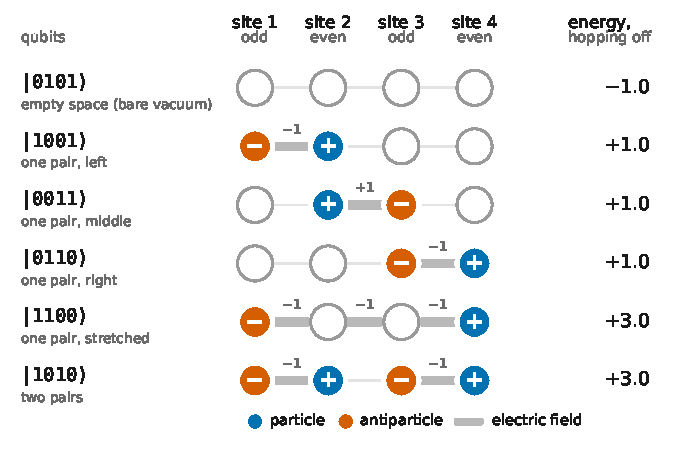
\includegraphics[width=0.72\textwidth]{13_lattice_states.pdf}
  \caption{The six bitstrings of zero total charge, with the charge on each
  site from Eq.~\eqref{eq:charge}, the field on each link from
  Eq.~\eqref{eq:gauss}, and the energy without hopping ($m = 0.5\,w$, $J = w$):
  $m$ per charge plus $J$ per unit of field on each link. Produced by
  \texttt{scripts/13\_lattice\_states.py}.}
  \label{fig:states}
\end{figure} With $\hat\rho_n = \tfrac12[\Zop{n} + (-1)^n]$ the Hamiltonian
becomes a spin chain, up to a constant that vanishes for even $N$,
\begin{equation}
  \label{eq:H}
  \Hop = \frac{m}{2}\sum_{n=1}^{N}(-1)^n \Zop{n}
       + w\sum_{n=1}^{N-1}\left(\sigp{n}\sigm{n+1} + \mathrm{h.c.}\right)
       + J\sum_{n=1}^{N-1}\Lop{n}^2,
  \qquad
  \Lop{n} = \frac12\sum_{k\le n}\left[\Zop{k} + (-1)^k\right].
\end{equation}

Expanded, Eq.~\eqref{eq:H} is a sum of Pauli strings, one Pauli matrix or
identity per qubit, written as words such as \texttt{ZIZI} read from site~1.
The hopping becomes $\tfrac12 w(\Xop{n}\Xop{n+1} + \Yop{n}\Yop{n+1})$. The
electric term couples each pair $k < k' \le N-1$ as
$\tfrac12 J (N - k')\,\Zop{k}\Zop{k'}$, so a neutral pair costs $J$ per link
between its charges: the linear potential on the lattice. Table~\ref{tab:pauli} lists the
fourteen strings at $N = 4$.

\begin{table}[t]
  \centering
  \caption{The $N=4$ Hamiltonian, Eq.~\eqref{eq:H}, as Pauli strings, leftmost
  character on site~1, printed by \texttt{scripts/03\_schwinger\_spectrum.py}.
  The three constructions of Section~\ref{sec:verification} agree exactly at
  these parameters and to \num{9e-16} or better at every other parameter set
  tried.}
  \label{tab:pauli}
  \small
  \begin{tabular}{llll}
    \toprule
    String & Coefficient & String & Coefficient \\
    \midrule
    \texttt{IIII} & $+2J$                      & \texttt{IIXX}, \texttt{IIYY} & $+\tfrac12 w$ \\
    \texttt{IIIZ} & $+\tfrac12 m$              & \texttt{IXXI}, \texttt{IYYI} & $+\tfrac12 w$ \\
    \texttt{IIZI} & $-\tfrac12 m - \tfrac12 J$ & \texttt{XXII}, \texttt{YYII} & $+\tfrac12 w$ \\
    \texttt{IZII} & $+\tfrac12 m - \tfrac12 J$ & \texttt{ZZII}                & $+J$ \\
    \texttt{ZIII} & $-\tfrac12 m - J$          & \texttt{ZIZI}, \texttt{IZZI} & $+\tfrac12 J$ \\
    \bottomrule
  \end{tabular}
\end{table}

\subsection{Parameters}
\label{sec:parameters}

All results use $N = 4$, $J = w$ and $m = 0.5\,w$, those of the main data set
of Martinez \emph{et al.}~\cite{martinez2016}, with time in units of $1/w$.
Since $J/w = (ag)^2$, this is $ag = 1$ and $m/g = 0.25$, a coarse lattice far
from the continuum limit, about which no claim is made.

\subsection{Symmetries that survive as diagnostics}
\label{sec:symmetries}

Gauss's law, $\Lop{n} - \Lop{n-1} - \hat\rho_n = 0$, holds identically in this
encoding (Section~\ref{sec:intro-diagnostic}), so diagnostics must come from
the two exact symmetries below. Both gate-noise models break them, but
logical-frame dephasing respects both (Section~\ref{sec:diagnostics}).

\emph{Total charge.} $\hat Q = \sum_n \hat\rho_n$ commutes with $\Hop$, so a
state stays in its charge sector, the bitstrings with a given $Q$. The bare
vacuum lies in the neutral sector: the six ``physical states'' Martinez
\emph{et al.}\ list~\cite{martinez2016}, those with two occupied sites.

\emph{CP inside the neutral sector.} CP is built from two lattice operations:
$\hat X^{\otimes N}$, which flips every qubit, and the mirror reflection $R$ of
site $n$ to $N+1-n$. Each alone also swaps the roles of odd and even sites,
turning $|0101\rangle$ into $|1010\rangle$, a state of different mean energy,
which an operator commuting with $\Hop$ could not do. In the product
$\mathrm{CP} = R\,\hat X^{\otimes N}$ the two swaps cancel, leaving charge
conjugation (particles exchanged with antiparticles) times parity (the mirror).
It moves each charge to the mirror site with its sign flipped,
$\hat\rho_n \to -\hat\rho_{N+1-n}$, and summing over the sites left of link $n$
gives
\begin{equation}
  \label{eq:cpL}
  \Lop{n} \to \Lop{N-n} - \hat Q ,
\end{equation}
the $-\hat Q$ arising because $\Lop{n}$ counts charge from the left end. The
mass and hopping terms are unchanged by CP in every sector, but the electric
term only when $Q = 0$: otherwise the cross term $-2\hat Q\Lop{N-n}$ survives.
CP therefore commutes with $\Hop$ in the neutral sector only. A neutral
state that CP leaves unchanged up to a phase, called CP-symmetric, therefore has
\begin{equation}
  \label{eq:cp}
  \langle \Lop{n} \rangle = \langle \Lop{N-n} \rangle .
\end{equation}
Neutrality alone is not enough: $|0110\rangle$ is neutral, but its links carry
$(0, 0, -1)$. CP returns the bare vacuum to itself, so every state evolved from
it is CP-symmetric too, and so is the ground state. Every factor of the Trotter
step conserves $\hat Q$ and commutes with CP in the neutral sector, so the
noiseless circuit keeps Eq.~\eqref{eq:cp} exactly at any step size, and a
violation larger than its shot-noise error bar comes from hardware error.

\subsection{Observables}
\label{sec:observables}

The physics observable is the particle density of Martinez
\emph{et al.}~\cite{martinez2016}, the mean number of particles plus
antiparticles per site,
\begin{equation}
  \label{eq:nu}
  \nu(t) = \frac{1}{2N}\sum_{n=1}^{N}\left[1 + (-1)^n\langle\Zop{n}(t)\rangle\right].
\end{equation}
It is zero on the bare vacuum, and at $N = 4$, $\nu = 1/2$ means one pair on
average. For
the ground state the observable is the chiral condensate
$\langle\bar\psi\psi\rangle = (2N)^{-1}\sum_n (-1)^n\langle\Zop{n}\rangle$, the
ground-state value, per site, of the operator that the mass multiplies. Since
$\nu = \tfrac12 + \langle\bar\psi\psi\rangle$, the density and the condensate
are the same operator up to a constant. The mass term is
$mN\bar\psi\psi$, so the Hellmann--Feynman theorem,
$dE_0/dm = \langle\partial\Hop/\partial m\rangle$, gives
$\langle\bar\psi\psi\rangle = N^{-1}\,dE_0/dm$ for the ground state.

The simulation starts in the bare vacuum, where the mass and electric terms are
at their minima, $-mN/2$ and zero. Forming pairs raises both, and since the
total energy is conserved exactly, the hopping term, initially zero, falls by
the same amount. At the first maximum of the density, $t = 0.89$, the mass and
electric terms have gained 0.93 and 0.97 and the hopping term has lost 1.90.

% ============================================================================
\section{Materials and Methods}
\label{sec:methods}
% ============================================================================

Every calculation in this thesis runs on a laptop. The quantum processor is
simulated on purpose, so that every intermediate quantity, including the full
noisy density matrix, can be inspected. The design rule is that each stage of
the pipeline has an answer known by independent means attached to it, and the
number reported for each check is a residual rather than a pass or fail flag.
Figure~\ref{fig:pipeline} shows the chain from the Hamiltonian to a measured
number, with the check attached at each link, and Table~\ref{tab:checks}
collects the residuals. This section describes each link in turn.

% ---------------------------------------------------------------- pipeline
\begin{figure}[t]
  \centering
  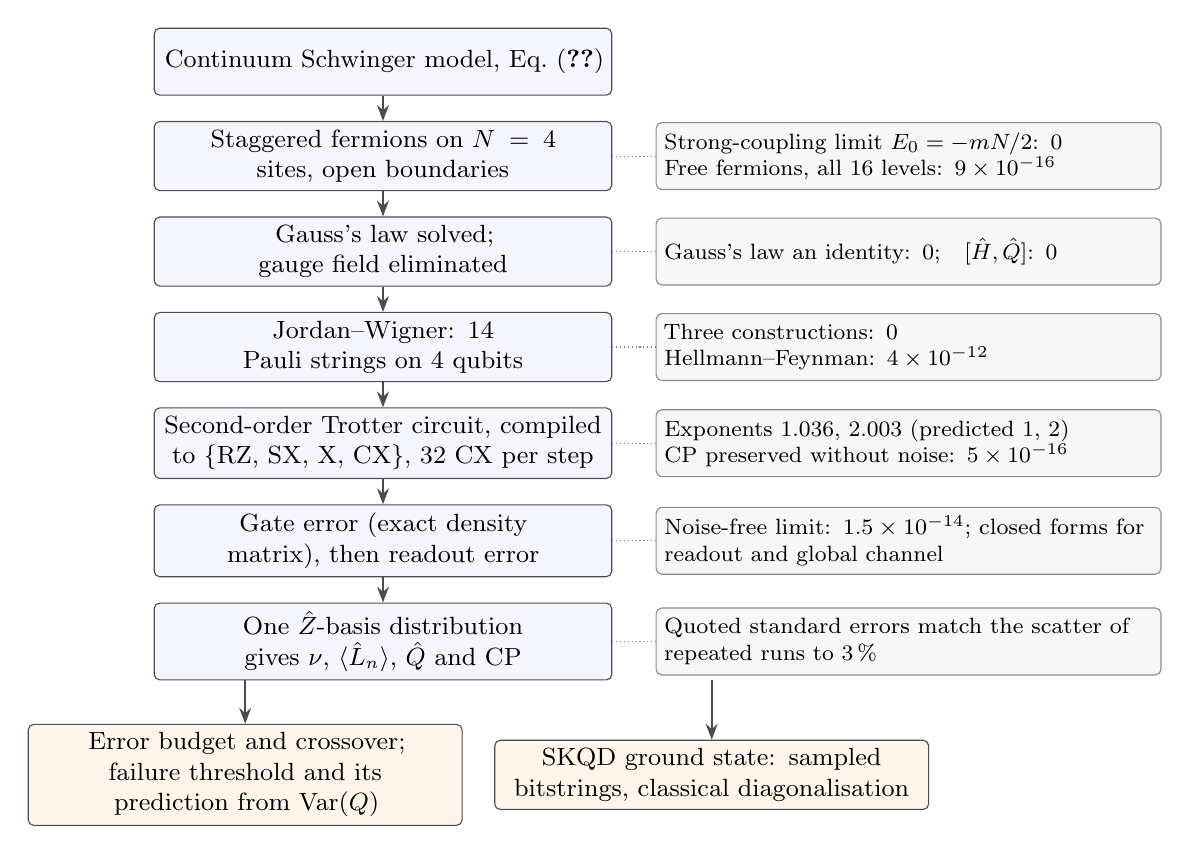
\begin{tikzpicture}[
      font=\small,
      nohyph/.style={execute at begin node={\hyphenpenalty=10000\exhyphenpenalty=10000}},
      box/.style={nohyph, draw=black!70, rounded corners=2pt, fill=blue!4, align=center,
                  text width=5.6cm, minimum height=0.85cm, inner sep=3pt},
      chk/.style={nohyph, draw=black!45, rounded corners=2pt, fill=black!3, align=left,
                  text width=6.2cm, minimum height=0.85cm, inner sep=3pt, font=\footnotesize},
      result/.style={nohyph, draw=black!70, rounded corners=2pt, fill=orange!8, align=center,
                  text width=5.3cm, minimum height=0.85cm, inner sep=3pt},
      flow/.style={-{Stealth[length=2mm]}, thick, black!70},
      link/.style={densely dotted, black!50},
      node distance=0.32cm]
    \node[box] (a) {Continuum Schwinger model, Eq.~\eqref{eq:lagrangian}};
    \node[box, below=of a] (b) {Staggered fermions on $N=4$ sites, open boundaries};
    \node[box, below=of b] (c) {Gauss's law solved; gauge field eliminated};
    \node[box, below=of c] (d) {Jordan--Wigner: 14 Pauli strings on 4 qubits};
    \node[box, below=of d] (e) {Second-order Trotter circuit, compiled to
                                $\{$RZ, SX, X, CX$\}$, 32 CX per step};
    \node[box, below=of e] (f) {Gate error (exact density matrix), then readout error};
    \node[box, below=of f] (g) {One $\Zop{}$-basis distribution gives
                                $\nu$, $\langle\Lop{n}\rangle$, $\hat Q$ and CP};
    \node[result, below=0.55cm of g, xshift=-1.75cm] (h) {Error budget and crossover;
                                failure threshold and its prediction from
                                $\mathrm{Var}(Q)$};
    \node[result, right=0.4cm of h] (i) {SKQD ground state: sampled bitstrings,
                                classical diagonalisation};
    \foreach \u/\v in {a/b, b/c, c/d, d/e, e/f, f/g} \draw[flow] (\u) -- (\v);
    \draw[flow] (g.south -| h.north) -- (h.north);
    \draw[flow] (g.south -| i.north) -- (i.north);

    \node[chk, right=0.55cm of b] (cb) {Strong-coupling limit $E_0=-mN/2$: 0\\
                                       Free fermions, all 16 levels: \num{9e-16}};
    \node[chk, right=0.55cm of c] (cc) {Gauss's law an identity: 0;\quad $[\Hop,\hat Q]$: 0};
    \node[chk, right=0.55cm of d] (cd) {Three constructions: 0\\
                                       Hellmann--Feynman: \num{4e-12}};
    \node[chk, right=0.55cm of e] (ce) {Exponents 1.036, 2.003 (predicted 1, 2)\\
                                       CP preserved without noise: \num{5e-16}};
    \node[chk, right=0.55cm of f] (cf) {Noise-free limit: \num{1.5e-14}; closed forms
                                       for readout and global channel};
    \node[chk, right=0.55cm of g] (cg) {Quoted standard errors match the scatter of
                                       repeated runs to 3\,\%};
    \foreach \u in {b, c, d, e, f, g} \draw[link] (\u) -- (c\u);
  \end{tikzpicture}
  \caption{The computational pipeline (left) and the independent check attached
  to each stage (right; residuals from Table~\ref{tab:checks}). The two outputs
  at the bottom are the dynamics error budget, with the crossover, the failure
  threshold and its prediction from charge conservation
  (Section~\ref{sec:budget-method}), and the ground state prepared by
  sample-based Krylov diagonalisation (Section~\ref{sec:skqd}), which reuses the
  same Trotter circuits.}
  \label{fig:pipeline}
\end{figure}

\subsection{Software}

The code is a Python 3.11 package, \texttt{schwinger}, with exact linear algebra
in NumPy~2.4 and SciPy~1.17~\cite{harris2020,virtanen2020}, circuits in
Qiskit~2.5~\cite{javadi2024}, noisy simulation in Qiskit Aer~0.17, and figures
in Matplotlib~3.11~\cite{hunter2007}; the exact versions are pinned in a lock
file. Each figure in this thesis is produced by one script that also prints the
residuals it relies on, every entry of Table~\ref{tab:checks} is printed by
\texttt{scripts/09\_verification\_table.py}, and all random sampling uses fixed
seeds, so rerunning a script reproduces its output. A suite of 476 tests
compares every module against independently known answers. The code, tests and
scripts are kept in a Git repository, private at the time of writing and
available from the author on request.

Two conventions cause silent errors if confused, and both are fixed in one
place in the code. A Pauli string such as \texttt{ZIZI} is read left to right as
site~1 to site~$N$, with site~1 the most significant tensor factor. Qiskit uses
the same label order but numbers its qubits in reverse, so lattice site $n$ is
Qiskit qubit $N-n$. Every gate index passes through a single conversion
function, and a test confirms that Qiskit's own operator, built from the labels
of Table~\ref{tab:pauli}, equals the NumPy matrix entry by entry.

\subsection{Exact reference and verification}
\label{sec:verification}

At $N = 4$ the Hamiltonian is a $16\times 16$ Hermitian matrix, diagonalised
exactly. Exact time evolution uses its spectral decomposition,
$|\psi(t)\rangle = \sum_k e^{-iE_k t}|k\rangle\langle k|\psi(0)\rangle$, so one
diagonalisation serves every time. These exact results are the reference for
every approximate result in the thesis, so the Hamiltonian itself is checked
first, in ways that fail for different reasons.

The matrix is built three ways that share nothing beyond the Pauli matrices
and the staggering sign $(-1)^n$: from the expanded Pauli list
of Table~\ref{tab:pauli}; directly, by squaring each $\Lop{n}$ as a matrix
without any algebra; and from the fermionic form Eq.~\eqref{eq:H_fermion}, with
fermion operators built through the Jordan--Wigner transformation. The three
agree to \num{9e-16} or better at every parameter set tried, and exactly at the
thesis parameters. This catches errors in the hand expansion of $\Lop{n}^2$ and
in the Jordan--Wigner signs, but not an error shared by all three, such as a
wrong starting Hamiltonian. Analytic limits test the physics instead. With no
hopping ($w = 0$) the Hamiltonian is diagonal and the bare vacuum minimises both
remaining terms, so $E_0 = -mN/2$ exactly; this tests the mass and electric
terms and is blind to the hopping. With no mass or field ($m = J = 0$) only the
hopping survives, a tight-binding chain with single-particle energies
$2w\cos[k\pi/(N+1)]$, $k = 1,\dots,N$, whose subset sums must reproduce all
sixteen levels; this tests the hopping and the Jordan--Wigner string and is
blind to the electric term.

A further check ties the observable to the Hamiltonian. The condensate computed
from the ground-state vector and the condensate computed as $N^{-1}dE_0/dm$ from
a finite difference of eigenvalues agree to \num{4e-12}, the size of the
finite-difference error. The Hellmann--Feynman theorem guarantees this
agreement for any Hamiltonian of the form $\Hop_0 + m\hat V$, so it shows only
that the observable and the mass term match in sign, staggering and
normalisation; the hopping and electric terms are covered by the constructions
and limits above. Before any of this, the Jordan--Wigner machinery was learned
on the transverse-field Ising model, whose full spectrum is known in closed
form~\cite{sachdev2011}; all $2^N$ levels were reproduced to \num{3e-14} for
$N = 2$, 4, 6 and 8. Finally, the Gauss's-law identity, $[\Hop,\hat Q] = 0$ and the
two CP maps of Section~\ref{sec:symmetries} are verified as operator identities
on the full space.

\begin{table}[tbp]
  \centering
  \caption{Verification checks at $N = 4$, $m = 0.5\,w$, $J = w$ unless stated,
  all printed by \texttt{scripts/09\_verification\_table.py}. Unless marked,
  each entry is the largest absolute disagreement between a computed quantity
  and an independently known answer, with energies in units of $w$; $0$ means
  exact agreement in floating point. Fitted exponents are given with their
  predicted values. Statistical checks are ratios of measured to predicted
  spread, which should be 1, or deviations in standard errors.}
  \label{tab:checks}
  \small
  \begin{tabular}{p{10.6cm}l}
    \toprule
    Check & Residual \\
    \midrule
    \multicolumn{2}{l}{\emph{Hamiltonian}} \\
    Pauli expansion vs.\ direct matrix construction & $0$ \\
    Fermionic form through Jordan--Wigner vs.\ spin form & $0$ \\
    Strong coupling, $E_0 = -mN/2$ at $w = 0$ & $0$ \\
    Free fermions, all 16 levels at $m = J = 0$ & \num{9e-16} \\
    Hellmann--Feynman: condensate vs.\ $N^{-1}dE_0/dm$ & \num{4e-12} \\
    Gauss's law as an operator identity; $[\Hop,\hat Q]$ & $0$; $0$ \\
    $[\mathrm{CP},\Hop]$ inside $Q = 0$ (largest element on the full space: 5) & $0$ \\
    CP maps $\hat\rho_n \to -\hat\rho_{N+1-n}$ and $\Lop{n} \to \Lop{N-n} - \hat Q$ & $0$; $0$ \\
    Drift of $\langle\Hop\rangle$ in exact evolution, $t \le 12$, $m/w = 0$ to 2 & \num{5e-15} \\
    Transverse-field Ising warm-up, full $2^N$ spectrum, $N = 2$, 4, 6, 8 & \num{3e-14} \\
    \midrule
    \multicolumn{2}{l}{\emph{Circuits}} \\
    Qiskit operator from Pauli labels vs.\ NumPy matrix & $0$ \\
    Circuit state vs.\ $e^{-i\Hop t}|\mathrm{vac}\rangle$ at $t = 2$, 4000 second-order steps & \num{7e-8} \\
    State-error exponent at $t = 3$, first / second order (predicted 1 / 2) & 1.036 / 2.003 \\
    Exponent of the bias on $\nu$ at $t = 1.76$, second order (predicted 2) & 2.002 \\
    Noiseless-circuit CP asymmetry, $\delta t = 0.5$, $0.25$, $0.1$, three times & \num{5e-16} \\
    \midrule
    \multicolumn{2}{l}{\emph{Noise}} \\
    Density-matrix simulation vs.\ statevector, no noise & \num{1.5e-14} \\
    Logical-frame route vs.\ Aer route, no noise & \num{2.9e-15} \\
    Infidelity convention vs.\ Qiskit's average gate fidelity (relative) & \num{4e-12} \\
    Readout: closed form $\tfrac12 + (1-2q)(\nu - \tfrac12)$, $q = 0.01$ to 0.2 & \num{6e-17} \\
    Readout: classical model vs.\ Aer, $q = 0.08$, $2\times10^5$ shots, worst bin & $1.9\,\sigma$ \\
    Global channel, $p = 0.005$ to 0.1 per step for 18 steps: $F_Q$ vs.\ $(1-p)^{18}$ & \num{7e-16} \\
    Logical-frame dephasing, $p = 0.01$, 0.05: $\mathrm{Var}(Q)$; $A_{\mathrm{CP}}$ (must vanish) & \num{9e-34}; \num{7e-16} \\
    Fully depolarising CX: $|\mathrm{Var}(Q) - N/4|$ & $0$ \\
    \midrule
    \multicolumn{2}{l}{\emph{Statistics, budget and ground state}} \\
    Scatter of 400 simulated runs / quoted standard error, $\nu$ and $\mathrm{Var}(Q)$ & 0.97 to 1.01 \\
    Mean squared error of 600 runs / $(b^2 + \sigma^2)$ & 0.999 \\
    Threshold prediction on data that obey the global model & \num{2e-16} \\
    Dip under four channels, $\delta t = 0.1$ to 0.3: largest $D - D_{\mathrm{noiseless}}$ (must be $< 0$) & \num{-2e-4} \\
    SKQD on the full neutral sector vs.\ exact ground energy & \num{4e-16} \\
    SKQD bound: smallest $E(S) - E_0$, 62 proper subspaces (must be $> 0$) & \num{3.2e-3} \\
    SKQD bias at 15 shots per step: exact / 20\,000 Monte Carlo runs
      & \num{1.020e-3} / \num{1.002(40)e-3} \\
    \bottomrule
  \end{tabular}
\end{table}

\subsection{Trotterised time evolution}

The Hamiltonian is split into three groups whose members commute among
themselves,
\begin{equation}
  \Hop = \Hop_Z + \Hop_{\mathrm{e}} + \Hop_{\mathrm{o}},
\end{equation}
where $\Hop_Z$ contains every $\Zop{}$ and $\Zop{}\Zop{}$ term (the mass and
electric energy, all diagonal), $\Hop_{\mathrm{e}}$ the hopping on the two outer
bonds, (1,2) and (3,4), and $\Hop_{\mathrm{o}}$ the hopping on the middle bond,
(2,3). The labels are the usual even and odd split with bonds counted from zero,
as in the code. Adjacent bonds share a site and do not commute, which is why the
hopping is split this way. Each group exponentiates exactly, so the only error
comes from the splitting. The first-order step is
$U_1(\delta t) = e^{-i\Hop_Z\delta t}e^{-i\Hop_{\mathrm{e}}\delta t}e^{-i\Hop_{\mathrm{o}}\delta t}$,
and the second-order, symmetric step used throughout is
\begin{equation}
  \label{eq:strang}
  U_2(\delta t) = e^{-i\Hop_Z\delta t/2}\,e^{-i\Hop_{\mathrm{e}}\delta t/2}\,
                  e^{-i\Hop_{\mathrm{o}}\delta t}\,
                  e^{-i\Hop_{\mathrm{e}}\delta t/2}\,e^{-i\Hop_Z\delta t/2}.
\end{equation}
A circuit to time $t$ applies the step $n$ times, with $n$ an integer, so a
nominal step $\delta t$ means $n = \mathrm{round}(t/\delta t)$ steps of $t/n$.
The error at fixed $t$ then scales as $\delta t$ for the first-order formula and
as $\delta t^2$ for the second~\cite{suzuki1976,childs2021}. The scaling is a
sharper test than the size of the error, because an implementation can be
accurate at one step size and still scale wrongly. The state error is defined
as the largest amplitude difference from $e^{-i\Hop t}|\mathrm{vac}\rangle$
after the global phase is removed. Fitting its logarithm against $\log\delta t$
at $t = 3$, for $\delta t$ from 0.3 to 0.0094, gives exponents of 1.036 and
2.003; the bias in the particle density at $t = 1.76$, for $\delta t$ from 0.088
to 0.011, gives 2.002.

Each exponential becomes gates directly. With the standard rotations
$\mathrm{R}_P(\theta) = e^{-i\theta P/2}$ for a Pauli operator $P$, a term
$c\,\Zop{n}$ is an $\mathrm{RZ}(2c\,\delta t)$ rotation and a term
$c\,\Zop{n}\Zop{n'}$ an $\mathrm{RZZ}(2c\,\delta t)$. On one bond,
$\tfrac12 w(\Xop{}\Xop{} + \Yop{}\Yop{})$ becomes $\mathrm{RXX}(w\,\delta t)$
followed by $\mathrm{RYY}(w\,\delta t)$; the two commute on the same bond, so
the pair is exact. For noise simulation the circuit is compiled to the native
gate set of superconducting devices, $\{\mathrm{RZ}, \mathrm{SX}, \mathrm{X},
\mathrm{CX}\}$, where SX is the square root of X and CX is the controlled-NOT
gate. In this set every RZZ, RXX and RYY costs two CX gates, and one
second-order step contains 32 CX, 24 SX and 53 RZ gates
(Figure~\ref{fig:trotterstep}). Compilation uses Qiskit's transpiler at
optimisation level 1 with a fixed seed and no coupling map, so any two qubits
are assumed to be directly coupled, as on a trapped-ion processor. On a chip
with nearest-neighbour coupling the RZZ between sites 1 and 3 would need extra
SWAP gates, and the CX counts here would rise. The RZ gates are implemented in
software on superconducting hardware, as a change of the phase reference of
later pulses, and carry no error~\cite{mckay2017}. The circuit whose gates are
counted and the circuit whose gates carry noise are the same compiled object.

\begin{figure}[t]
  \centering
  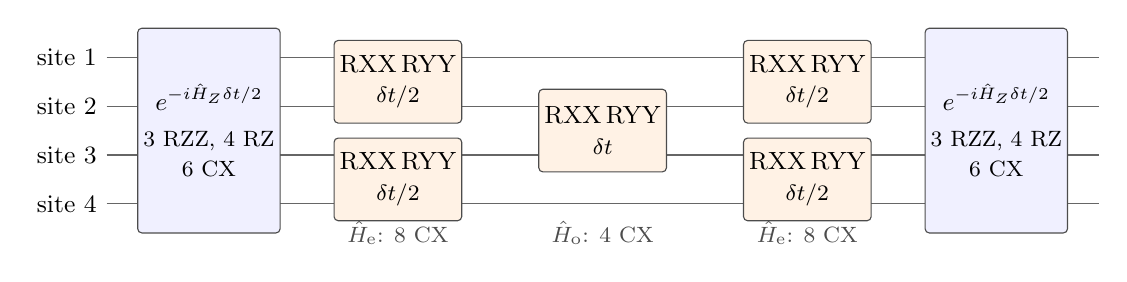
\begin{tikzpicture}[font=\small, x=1cm, y=0.62cm,
      gate/.style={draw=black!70, fill=white, rounded corners=1.5pt, align=center,
                   minimum width=1.55cm, inner sep=2pt},
      diag/.style={gate, fill=blue!6},
      hop/.style={gate, fill=orange!10}]
    \foreach \q in {1,...,4} {
      \draw[black!60] (0,-\q) -- (12.6,-\q);
      \node[left] at (0,-\q) {site \q};
    }
    \node[diag, minimum height=2.6cm] at (1.3,-2.5)
      {$e^{-i\Hop_Z\delta t/2}$\\[2pt]\footnotesize 3 RZZ, 4 RZ\\\footnotesize 6 CX};
    \node[hop, minimum height=1.05cm] at (3.7,-1.5) {RXX\,RYY\\\footnotesize $\delta t/2$};
    \node[hop, minimum height=1.05cm] at (3.7,-3.5) {RXX\,RYY\\\footnotesize $\delta t/2$};
    \node[hop, minimum height=1.05cm] at (6.3,-2.5) {RXX\,RYY\\\footnotesize $\delta t$};
    \node[hop, minimum height=1.05cm] at (8.9,-1.5) {RXX\,RYY\\\footnotesize $\delta t/2$};
    \node[hop, minimum height=1.05cm] at (8.9,-3.5) {RXX\,RYY\\\footnotesize $\delta t/2$};
    \node[diag, minimum height=2.6cm] at (11.3,-2.5)
      {$e^{-i\Hop_Z\delta t/2}$\\[2pt]\footnotesize 3 RZZ, 4 RZ\\\footnotesize 6 CX};
    \node[font=\footnotesize, black!70] at (3.7,-4.6) {$\Hop_{\mathrm{e}}$: 8 CX};
    \node[font=\footnotesize, black!70] at (6.3,-4.6) {$\Hop_{\mathrm{o}}$: 4 CX};
    \node[font=\footnotesize, black!70] at (8.9,-4.6) {$\Hop_{\mathrm{e}}$: 8 CX};
  \end{tikzpicture}
  \caption{One second-order Trotter step, Eq.~\eqref{eq:strang}, on four
  qubits. Diagonal layers (blue) apply the mass and electric terms. Hopping
  layers (orange) apply $\tfrac12 w(\Xop{}\Xop{}+\Yop{}\Yop{})$ to the outer bonds
  for half a step, the middle bond for a full step, and the outer bonds again.
  Compiled to $\{\mathrm{RZ},\mathrm{SX},\mathrm{X},\mathrm{CX}\}$ the step costs
  32 CX gates, the number that sets how fast gate error accumulates.}
  \label{fig:trotterstep}
\end{figure}

\subsection{Measurement and shot noise}

Every observable in Section~\ref{sec:theory}, together with $\hat Q$, is
diagonal in the computational basis, so each is a function $x_b$ of the measured
bitstring $b$ alone. One circuit measured once in the $\Zop{}$ basis therefore
gives the physics and the diagnostics together, with no extra circuits. An
$M$-shot estimate of $\langle x\rangle$ is the sample mean, and its standard
error is
\begin{equation}
  \label{eq:sigma}
  \sigma_x = \sqrt{\frac{1}{M}\sum_b p_b\,\bigl(x_b - \langle x\rangle\bigr)^2},
  \qquad \langle x\rangle = \sum_b p_b x_b ,
\end{equation}
where $p_b$ is the probability of outcome $b$~\cite{taylor1997}. The particle
number of a single shot takes the values 0, 1, 2, 3 or 4, not just 0 and 1, so
the binomial formula $\sqrt{p(1-p)/M}$ does not apply and Eq.~\eqref{eq:sigma}
is the general form. For $\mathrm{Var}(Q)$ the standard error of a sample
variance is used, $\sqrt{(\mu_4 - \mu_2^2)/M}$, with $\mu_2 = \mathrm{Var}(Q)$
and $\mu_4$ the second and fourth central moments of $Q$ per shot.

The distribution $p_b$ is known exactly in simulation, so Eq.~\eqref{eq:sigma} is
evaluated exactly rather than estimated from one noisy sample, and shot noise
enters the budget as a computed number rather than as a fluctuation that has to
be averaged away. When a realistic data set is needed, $M$ outcomes are drawn
from $p_b$ by multinomial sampling, which is statistically identical to running
the circuit $M$ times. Over 400 independent simulated data sets of 256 and of
2048 shots, the actual scatter of the estimates is between 0.97 and 1.01 times
the quoted standard error, for both $\nu$ and $\mathrm{Var}(Q)$.

\subsection{Hardware noise models}

Gate errors are modelled as depolarising channels attached to the physical
gates of the compiled circuit. Acting on the $d$-dimensional space of a gate's
own qubits,
\begin{equation}
  \mathcal{E}(\rho) = (1-\lambda)\,\rho + \lambda\,\frac{I_d}{d}\otimes\mathrm{Tr}_g\,\rho,
\end{equation}
where $\mathrm{Tr}_g$ traces out those qubits, $d = 4$ for a CX gate and $d = 2$
for SX and X. The strength is quoted as the average gate infidelity $\epsilon$,
the number obtained from randomised benchmarking and reported on hardware data
sheets~\cite{magesan2011}, which is related to $\lambda$ by
$\epsilon = \lambda(d-1)/d$~\cite{nielsen2010,magesan2011}. Confusing the two
would misstate every threshold by a factor $4/3$, so the conversion is checked
against Qiskit's own average-gate-fidelity routine. The two-qubit error
$\epsilon_2$ is swept from $10^{-5}$ to $3\times 10^{-2}$, a range that brackets
the two-qubit error of $4\times10^{-3}$ reported for the trapped-ion processor
used by Rosanowski \emph{et al.}~\cite{rosanowski2025}. The single-qubit error
is set to $\epsilon_1 = \epsilon_2/10$. This ratio is an assumption. With it,
the 24 SX gates of each step add less than a tenth of the error that its 32 CX
gates do, and its effect on the failure threshold defined below is tested by
repeating the threshold sweep with $\epsilon_1 = 0$ and
$\epsilon_1 = 0.3\,\epsilon_2$.

As a control, the CX depolarising channel is replaced in some runs by
independent phase flips, $\rho \to (1-\epsilon_2)\rho + \epsilon_2\Zop{}\rho\Zop{}$
on each of its two qubits, with flips of probability $\epsilon_1$ after SX and
X. Here $\epsilon_2$ is a flip probability, not an average infidelity, so the
two models are compared through the fidelity they produce, Eq.~\eqref{eq:FQ}
below, and not at equal $\epsilon_2$.

Readout error is modelled as an independent bit flip with probability $q$ on
each qubit, applied as a $2\times 2$ confusion matrix to each qubit's axis of the
outcome distribution. It acts only on the classical record, after the state has
been measured, so it is applied afterwards to the computed noisy distribution and its
bias stays separate from the gate error. A symmetric flip maps every
$\langle\Zop{n}\rangle$ to $(1-2q)\langle\Zop{n}\rangle$, so the particle density
becomes $\tfrac12 + (1-2q)(\nu - \tfrac12)$; the code reproduces this closed form
to \num{6e-17}, and over $2\times 10^5$ sampled shots it agrees with Aer's own
readout-error model to within $1.9$ standard deviations in every outcome bin.
Readout error can be corrected by inverting the confusion
matrix~\cite{bravyi2021}, so it is reported as its own term in the budget rather
than folded into the gate error.

The noisy state is computed exactly. Aer's density-matrix simulator carries the
full $16\times 16$ density matrix through every noisy gate and returns the exact
outcome probabilities, with no sampling. The gate-error bias of any observable is
then an exact number, and shot noise is added afterwards through
Eq.~\eqref{eq:sigma}.

A second route applies noise once per Trotter step to the state of the four
lattice sites, called here the logical frame to distinguish it from errors
inside a compiled gate. The step unitary is taken as a $16\times16$ matrix and
the noise is applied with NumPy matrix products, bypassing Aer and the
transpiler. This logical-frame route implements the phenomenological model
Martinez \emph{et al.}\ fitted to their data, a phase flip with probability $p$
on each qubit per step~\cite{martinez2016}, and a global depolarising channel
$\rho \to (1-p)\rho + pI/16$ per step. At zero noise it agrees with the Aer
route to \num{2.9e-15}. It exists as a control for the diagnostics, for the
reason given in Section~\ref{sec:diagnostics}. Four kinds of noise strength
appear and are kept apart: the average infidelity $\epsilon$ of a gate
($\lambda$ is its channel parameter), the readout flip probability $q$, the
probability $p$ per Trotter step of the logical-frame channels, and the
fidelity $F$ of a whole circuit.

Not modelled are amplitude damping, coherent errors such as a systematically
over-rotated gate, and errors correlated between qubits or between steps.
Amplitude damping drives every qubit toward $|0\rangle$, an occupied site here,
and its end point $|0000\rangle$ is a pure state with $Q = 2$ and
$\mathrm{Var}(Q) = 0$, so the global-model reading of $\mathrm{Var}(Q)$ in the
next subsection would fail for it.

\subsection{Symmetry diagnostics}
\label{sec:diagnostics}

From the same $\Zop{}$-basis data, three diagnostics are computed: the charge
variance $\mathrm{Var}(Q) = \langle\hat Q^2\rangle - \langle\hat Q\rangle^2$,
the leakage $1 - P(Q = 0)$ out of the six-state neutral sector, which is the
quantity Martinez \emph{et al.}\ reported~\cite{martinez2016}, and the CP
asymmetry $A_{\mathrm{CP}} = \langle\Lop{1}\rangle - \langle\Lop{3}\rangle$.
Without hardware noise all three vanish exactly, at any step size, because
every factor of the Trotter step conserves $\hat Q$ and commutes with CP in the
neutral sector (Section~\ref{sec:symmetries}).

Turning a violation into a prediction needs a model of the noise. The simplest
is a global depolarising channel, $\rho \to F\rho + (1-F)I/16$, under which every
diagonal observable moves linearly toward its maximally mixed value with the
same weight $F$~\cite{vovrosh2021,urbanek2021}. The ideal state has
$\mathrm{Var}(Q) = 0$ and the maximally mixed state has $\mathrm{Var}(Q) = N/4$,
so the model gives
\begin{equation}
  \label{eq:FQ}
  F_Q = 1 - \frac{\mathrm{Var}(Q)}{N/4},
\end{equation}
and an analogous estimate from the leakage. Both are exact for a global channel.
Real gate noise is local, not global, so Eq.~\eqref{eq:FQ} is a model whose
accuracy is one of the things this thesis measures. Only the charge variance is
turned into a prediction. The CP asymmetry vanishes on the maximally mixed
state, where $\langle\Lop{1}\rangle = \langle\Lop{3}\rangle = -\tfrac12$, so a
global channel cannot move it and it has no analogue of Eq.~\eqref{eq:FQ};
under gate noise it first grows and then returns to zero. It is reported as a
check and is not used as a predictor.

The diagnostics have a blind spot, and the logical-frame route exposes it. A
$\Zop{}$ error on the logical state commutes with $\hat Q$, so dephasing between
Trotter steps leaves $\mathrm{Var}(Q)$ exactly zero while the particle density
drifts far from its noiseless value. Uniform dephasing also commutes with CP,
so the CP asymmetry stays zero as well. Dephasing on the CX gates of the compiled
circuit, by contrast, does break charge conservation: a compiled RXX or RYY is
wrapped in single-qubit basis changes, so its CX gates act in a rotated frame,
and a $\Zop{}$ error on either of them becomes an $\Xop{}$ or $\Yop{}$ error on
the logical state. Whether an error is visible to the diagnostic therefore
depends on where in the compiled circuit it occurs as well as on its type.

\subsection{The error budget}
\label{sec:budget-method}

For a diagonal observable at time $t$ and step size $\delta t$, four outcome
distributions are computed exactly, each differing from the last by one source of
error: $p^{\mathrm{exact}}$ from $e^{-i\Hop t}$, $p^{\mathrm{Trot}}$ from the
noiseless circuit, $p^{\mathrm{gate}}$ from the same circuit with gate noise, and
$p^{\mathrm{meas}}$ after readout error. The biases telescope,
\begin{equation}
  \label{eq:budget}
  \langle x\rangle^{\mathrm{meas}} - \langle x\rangle^{\mathrm{exact}}
  = b_{\mathrm{Trot}} + b_{\mathrm{gate}} + b_{\mathrm{read}},
\end{equation}
with $b_{\mathrm{Trot}} = \langle x\rangle^{\mathrm{Trot}} - \langle x\rangle^{\mathrm{exact}}$,
$b_{\mathrm{gate}} = \langle x\rangle^{\mathrm{gate}} - \langle x\rangle^{\mathrm{Trot}}$
and $b_{\mathrm{read}} = \langle x\rangle^{\mathrm{meas}} - \langle x\rangle^{\mathrm{gate}}$,
so the three biases add to the total exactly, by construction. The split itself
is a choice. Because the gate bias is defined on the Trotterised circuit, any
interplay between Trotter and gate error is counted as gate error, which matches
how an experiment is designed: the circuit is fixed first and then run on noisy
hardware. The shot noise $\sigma$ follows from $p^{\mathrm{meas}}$ through
Eq.~\eqref{eq:sigma}, and the root-mean-square error of a single $M$-shot
measurement is $\sqrt{b^2 + \sigma^2}$, with $b$ the total bias: the mean
squared error of an estimator is its squared bias plus its
variance~\cite{cai2023}. As a check that the estimator, the sampling code and
Eq.~\eqref{eq:sigma} agree with one another, 600 simulated 500-shot experiments
at $\epsilon_2 = 10^{-3}$ and $q = 0.02$ have a mean squared deviation from the
exact answer of 0.999 times $b^2 + \sigma^2$. Because the samples are drawn from
the same $p^{\mathrm{meas}}$, this confirms the bookkeeping, not the
completeness of the noise model.

Two times recur below. Starting from the bare vacuum, the exact particle density
rises to its first maximum, $\nu = 0.463$ at $t_{\mathrm{p}} = 0.89$, and falls to
its first minimum, $\nu = 0.133$ at $t_{\mathrm{t}} = 1.76$, as pairs recombine.

\emph{The crossover.} The crossover step $\delta t_\times$ is the step at which
the Trotter bias in $\nu(t)$, with no hardware error, falls to the shot-noise
uncertainty $\sigma(M)$ of Eq.~\eqref{eq:sigma}, computed from the full outcome
distribution rather than sampled. It is located by
linear interpolation in $\log\delta t$ between neighbouring grid points
$\delta t = t/n$, at $t = 3$ (every $n$ from 2 to 32, then coarser up to 256)
and at $t_{\mathrm{t}}$ (14 values of $n$ from 2 to 64), for $M = 256$, 1000 and
4096 shots.

\emph{The optimal step.} For a 1000-shot measurement of $\nu(t_{\mathrm{t}})$
with readout error $q = 0.01$, the error $\sqrt{b^2 + \sigma^2}$ is evaluated on
the same 14 step sizes at $\epsilon_2 = 0$, $3\times10^{-4}$, $10^{-3}$ and
$3\times10^{-3}$, and the optimum is the grid point with the smallest error. At
the optimum, the share of each source is its square divided by
$b_{\mathrm{Trot}}^2 + b_{\mathrm{gate}}^2 + b_{\mathrm{read}}^2 + \sigma^2$,
for $\nu$ and for the outer and middle link fields.

\emph{The failure threshold.} The signal is the recombination dip
\begin{equation}
  \label{eq:dip}
  D = \nu(t_{\mathrm{p}}) - \nu(t_{\mathrm{t}}),
  \qquad
  \sigma_D = \sqrt{\sigma_{\mathrm{p}}^2 + \sigma_{\mathrm{t}}^2}.
\end{equation}
Depolarising noise drives the state toward the maximally mixed state, where
$\nu = \tfrac12$ at every time and $D = 0$. In every noise sweep in this thesis,
for each of the four channels modelled and all three step sizes, $D$ shrinks
from its noiseless value as the noise grows, and can fall below zero, but never
exceeds that value (Table~\ref{tab:checks}); a dip that survives was therefore
not created by the noise. This is an observation about the channels modelled
rather than a theorem. Coherent errors, which are not modelled, could in
principle shift or mimic the dip. The failure threshold $\epsilon^\ast$ is the smallest two-qubit error at
which $D \le 2\sigma_D$, found by interpolation in $\log\epsilon_2$ on a
36-point grid from $10^{-5}$ to $3\times10^{-2}$, for nominal step sizes
$\delta t = 0.1$, $0.2$ and $0.3$ and for $M = 10^3$ and $10^4$ shots. The number
of steps is rounded separately at each time; for $\delta t = 0.2$ that is four
steps to $t_{\mathrm{p}}$ and nine to $t_{\mathrm{t}}$. The measurement times
are fixed at the extrema of the exact evolution, as an experiment would choose
them from theory. Readout error is left out of the threshold and of its
prediction. It would add about $Nq(1-q)$, roughly 0.04 at $q = 0.01$, to
$\mathrm{Var}(Q)$ and multiply $D$ by $1-2q$, so on hardware the confusion
matrix would have to be inverted before Eq.~\eqref{eq:FQ} is applied.

\emph{Predicting the threshold.} An experiment has data at one noise level
$\epsilon_0$ only, and the prediction uses those data alone, in four steps.
First, Eq.~\eqref{eq:FQ} turns the measured charge variance into a fidelity
$F_Q$ at each of the two measurement times. Second, the global model is
assumed, so the measured distribution $p$ is inverted to an estimate of the
ideal one, $p^{\mathrm{ideal}} = [p - (1-F_Q)/16]/F_Q$. Third, the fidelity is
assumed to decay exponentially with gate error, $F(\epsilon) =
e^{-\kappa\epsilon}$, with $\kappa = -\ln F_Q/\epsilon_0$ fixed separately at
each time. Fourth, $p^{\mathrm{ideal}}$ is degraded with $F(\epsilon)$ at every
other $\epsilon$ to predict $D$ and $\sigma_D$ there, and the crossing of the
predicted $D$ with $2\sigma_D$ is the predicted threshold. Nothing in this
procedure uses the exact answer, and on synthetic data that obey the global
model it reproduces the true dip to \num{2e-16}. In the main comparison
$\mathrm{Var}(Q)$ at $\epsilon_0$ is computed from the full, unsampled noisy
distribution, so the test isolates the error of the global model from the shot noise on the
diagnostic. A real experiment would have $M$-shot data at $\epsilon_0$, so the
prediction is repeated on 200 data sets of 1000 shots sampled from that
distribution, which gives the scatter a single run would show. Comparing the
prediction with the threshold found by sweeping $\epsilon_2$ directly, for
$\epsilon_0$ near $\epsilon^\ast/10$ and $\epsilon^\ast/3$, is the test of the
third question in Section~\ref{sec:contribution}. The same comparison is
repeated with dephasing on the CX gates, the second gate-noise model.

\subsection{Ground state by sample-based Krylov diagonalisation}
\label{sec:skqd}

The ground state is prepared with SKQD, following Yu
\emph{et al.}~\cite{yu2025} and its application to the Schwinger model by
Rosanowski \emph{et al.}~\cite{rosanowski2025}. The reference state is the bare
vacuum, the ground state of the mass and electric terms, which Rosanowski
\emph{et al.}\ use as the initial state for their runs up to 30 qubits. The
circuits prepare $U(\delta t)^k|\mathrm{vac}\rangle$ for $k = 1,\dots,K$, with
$U(\delta t)$ either one second-order Trotter step of the full Hamiltonian,
Eq.~\eqref{eq:strang}, which reuses the dynamics circuits directly, or a step of
the hopping terms alone, of the kind Rosanowski \emph{et al.}\ use. Each circuit
is measured $M$ times. Bitstrings with nonzero total charge are discarded, which
costs nothing because $\hat Q$ is diagonal, and the distinct neutral bitstrings
from all $K$ steps, together with the reference, form a set $S$. The
Hamiltonian restricted to the span of $S$ is diagonalised classically, and its
lowest eigenvalue and eigenvector give the energy and the chiral condensate.
Because this is an exact diagonalisation inside a subspace, the estimate
satisfies $E_{\mathrm{SKQD}} \ge E_0$ for every possible $S$, however noisy the
sampling~\cite{kanno2023}. The bound holds on all 63 nonempty subsets of the
neutral sector, with a smallest margin of \num{3.2e-3} among the 62 proper ones.

Noise therefore cannot push the energy below the truth, but a finite number of
shots can miss an important bitstring and push it above~\cite{miura2026}. At
$N = 4$ this bias can be computed exactly. Let $p_k(b)$ be the outcome
distribution of the $k$-th circuit. For the sampled set to lie inside a set $T$
of neutral bitstrings, every one of the $M$ shots at every step must avoid the
neutral bitstrings outside $T$, so
\begin{equation}
  \label{eq:skqd}
  P(S \subseteq T) = \prod_{k=1}^{K}\Bigl(1 - \sum_{b \notin T} p_k(b)\Bigr)^{M}
\end{equation}
for every $T$ that contains the reference, and zero otherwise. The sum runs
over neutral bitstrings only; shots on charged bitstrings are discarded and do
no harm. Inclusion and exclusion over the $2^6 = 64$ subsets of the neutral
sector convert Eq.~\eqref{eq:skqd} into the probability that the sampled set is
exactly $S$, and the expected SKQD energy is the probability-weighted average of
the subspace energies. This exact result agrees with 20\,000 simulated SKQD runs
(Table~\ref{tab:checks}) and replaces Monte Carlo averaging in everything that
follows.

The hopping-only step needs one caution. Rosanowski \emph{et al.}\ write it as
$\exp[i(dt/4)\sum_n(\Xop{n}\Xop{n+1} + \Yop{n}\Yop{n+1})]$, which turns each
bond half as far as $\mathrm{RXX}(w\,\delta t)\,\mathrm{RYY}(w\,\delta t)$ does
at the same number, and their four-qubit run started from $|0011\rangle$ at
different parameters~\cite{rosanowski2025}. The SKQD runs therefore use
both $w\,\delta t = 0.77$, the value they chose, and $w\,\delta t = 0.385$, the
rotation it gives in their convention, and the comparison is with the kind of
step they use rather than with their circuit.

\subsection{Simulation parameters}

The physical parameters are those of Section~\ref{sec:parameters} and the
initial state is the bare vacuum. Trotter steps are second order unless stated
otherwise. The scaling test uses $\delta t$ from 0.0094 to 0.3 at $t = 3$. The
crossover uses $\delta t$ from 0.012 to 1.5 at $t = 3$ and, together with the
full budget, from 0.028 to 0.88 at $t_{\mathrm{t}}$. The threshold uses nominal
steps $\delta t = 0.1$, 0.2 and 0.3. Shot counts run from 256 to $10^4$ for the
dynamics and from 2 to 500 per Krylov step for SKQD; two-qubit gate errors run
from $10^{-5}$ to $3\times10^{-2}$ with $\epsilon_1 = \epsilon_2/10$; the
readout error in the budget is $q = 0.01$. SKQD uses $K = 4$ full Trotter steps
of $\delta t = 0.3$, without gate error and with $\epsilon_2 = 3\times10^{-3}$,
and a single hopping-only step of $w\,\delta t = 0.77$ or 0.385.

% ============================================================================
\section{Results}
\label{sec:results}
% ============================================================================
% FIRST DRAFT, written 2026-10-13 from scripts 04 to 08. Every number below is
% printed by the script named next to it; rerun the script before trusting a
% number here.

\subsection{Pair production from the bare vacuum}

Figure~\ref{fig:pairs} shows the particle density after a quench from the bare
vacuum, computed exactly. Energy is conserved to \num{4e-15} throughout and the
total charge never leaves zero. Nothing is injected: the bare vacuum is not an
eigenstate of the full Hamiltonian, and the energy it already holds moves between
the electric field and the rest mass of the pairs. Table~\ref{tab:quench} makes
this quantitative. The larger the gap between the energy of the bare vacuum and
the true ground-state energy, the more pairs appear, and the relation is
monotone across the four masses studied. The two outer links carry identical
flux at every time, $|\langle\Lop{1}\rangle - \langle\Lop{3}\rangle| <
\num{1e-15}$, as the CP symmetry of Eq.~\eqref{eq:cp} requires.

\begin{figure}[t]
  \centering
  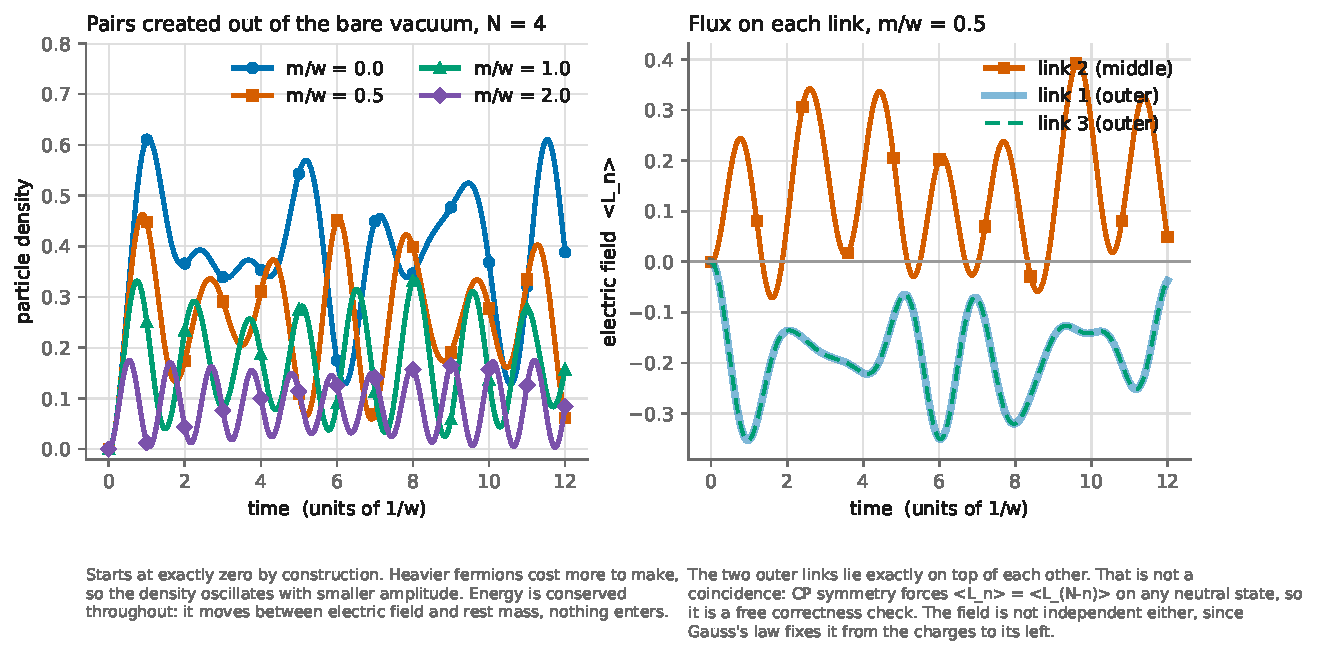
\includegraphics[width=\textwidth]{04_pair_production.pdf}
  \caption{Left: particle density against time after a quench from the bare
  vacuum, for four fermion masses, computed exactly. Right: the electric field
  on each link at $m = 0.5\,w$; the two outer links coincide, as CP requires.
  Produced by \texttt{scripts/04\_pair\_production\_preview.py}.}
  \label{fig:pairs}
\end{figure}

\begin{table}[t]
  \centering
  \caption{Why pairs appear. $E_{\mathrm{bare}}$ is the energy of the bare
  vacuum, $E_0$ the exact ground-state energy, and $\nu_{\max}$ the largest
  particle density reached for $0 \le t \le 12$ ($J = w$).}
  \label{tab:quench}
  \small
  \begin{tabular}{ccccc}
    \toprule
    $m/w$ & $E_{\mathrm{bare}}$ & $E_0$ & $E_{\mathrm{bare}} - E_0$ & $\nu_{\max}$ \\
    \midrule
    0.0 & $\phantom{-}0.000$ & $-1.477$ & 1.477 & 0.612 \\
    0.5 & $-1.000$ & $-2.075$ & 1.075 & 0.463 \\
    1.0 & $-2.000$ & $-2.828$ & 0.828 & 0.335 \\
    2.0 & $-4.000$ & $-4.553$ & 0.553 & 0.175 \\
    \bottomrule
  \end{tabular}
\end{table}

\subsection{Trotter error against shot noise: the crossover}

The Trotter error scales with the predicted exponents (Figure~\ref{fig:trotter},
left), so its size at any step can be trusted. Figure~\ref{fig:trotter} (right)
compares the Trotter bias in the particle density at $t = 3$ with the shot-noise
uncertainty. The standard error is \num{0.0176} at 256 shots and \num{0.0047} at
4096, and the Trotter bias falls below these floors at $\delta t \approx 0.19$
and $\delta t \approx 0.094$ respectively. At the first recombination minimum,
$t = 1.76$, the crossover sits at $\delta t = 0.44$, $0.35$ and $0.22$ for 256,
1000 and 4096 shots (\texttt{scripts/08}). Below the crossover a smaller step
buys accuracy the statistics cannot resolve, while the circuit keeps growing:
the two-qubit gate count at $t = 3$ rises from 320 at $\delta t = 0.3$ to 6400
at $\delta t = 0.015$.

\begin{figure}[t]
  \centering
  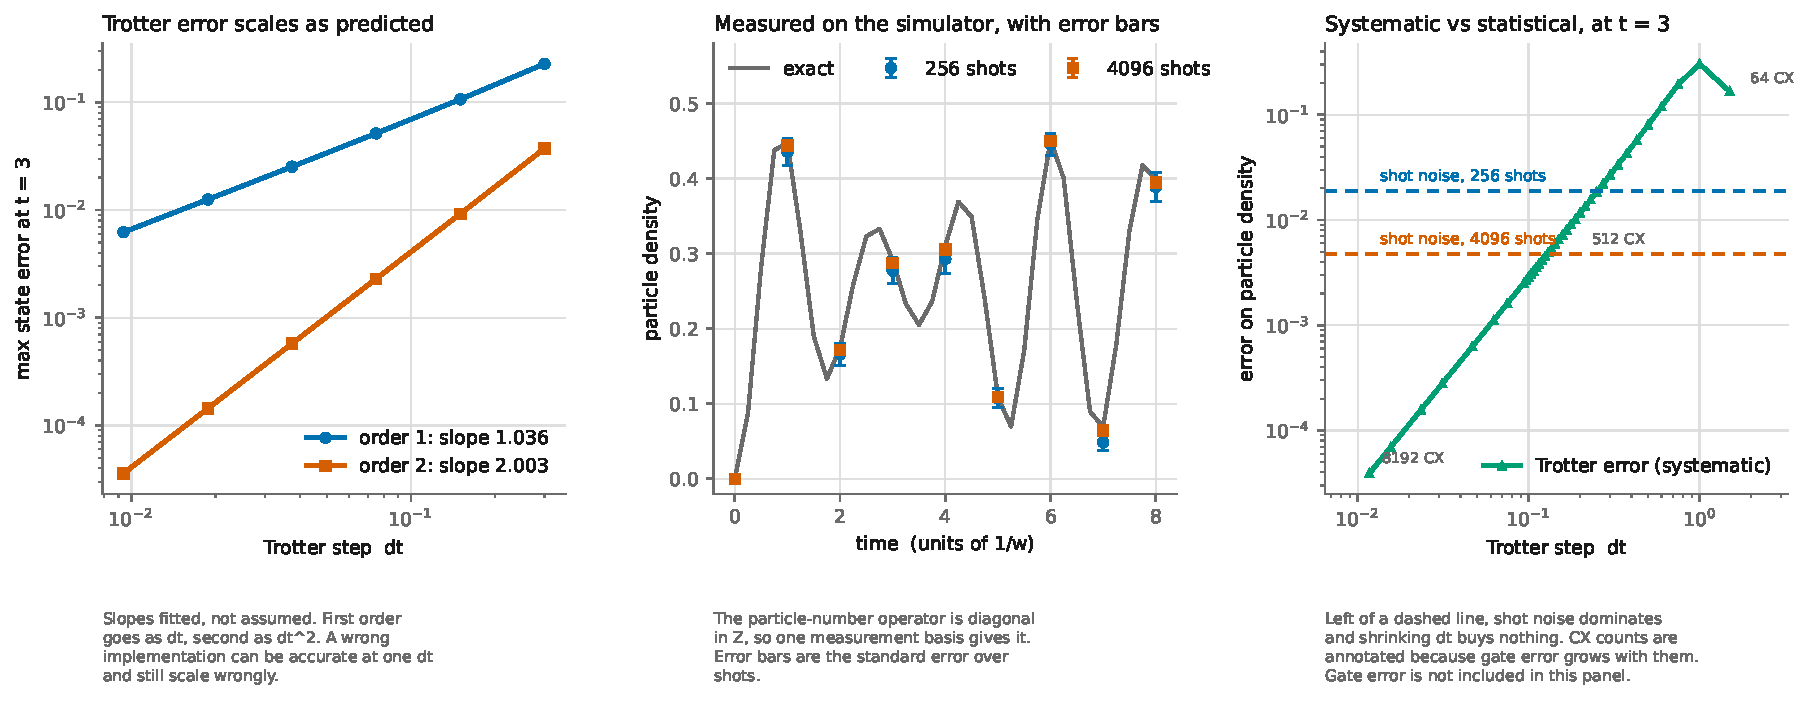
\includegraphics[width=\textwidth]{05_qiskit_trotter.pdf}
  \caption{Left: Trotter error against step size, with the scaling exponent
  fitted rather than assumed. Centre: particle density measured from finite
  shots. Right: the crossover between Trotter bias and shot noise at $t = 3$.
  Produced by \texttt{scripts/05\_qiskit\_trotter.py}.}
  \label{fig:trotter}
\end{figure}

\subsection{Gate error and the failure threshold}

Figure~\ref{fig:threshold}(a) shows what depolarising gate error does to the
pair-production signal at $\delta t = 0.1$. The density is pulled toward the
maximally mixed value $\tfrac12$, the later times first, because their circuits
are deeper. At $\epsilon_2 = 10^{-3}$ the recombination dip keeps about half its
noiseless size; at $\epsilon_2 = 10^{-2}$ it is gone.
Figure~\ref{fig:threshold}(b) and Table~\ref{tab:threshold} give the failure
threshold for three step sizes.

\begin{table}[t]
  \centering
  \caption{Failure threshold $\epsilon^\ast$, the two-qubit error at which the
  recombination dip falls to twice its shot-noise uncertainty, with
  $\epsilon_1 = \epsilon_2/10$. $n_{\mathrm{CX}}$ is the CX count of the deeper
  (trough) circuit. From \texttt{scripts/06\_noise\_threshold.py}.}
  \label{tab:threshold}
  \small
  \begin{tabular}{cccccc}
    \toprule
    $\delta t$ & $n_{\mathrm{CX}}$ & $\epsilon^\ast$ ($10^3$ shots) & $\epsilon^\ast n_{\mathrm{CX}}$
      & $\epsilon^\ast$ ($10^4$ shots) & $\epsilon^\ast$ (no shot noise) \\
    \midrule
    0.1 & 576 & \num{3.3e-3} & 1.92 & \num{4.0e-3} & \num{4.6e-3} \\
    0.2 & 288 & \num{6.9e-3} & 1.98 & \num{8.4e-3} & \num{9.4e-3} \\
    0.3 & 192 & \num{1.06e-2} & 2.03 & \num{1.29e-2} & \num{1.45e-2} \\
    \bottomrule
  \end{tabular}
\end{table}

The threshold is set by circuit depth. At 1000 shots the product
$\epsilon^\ast n_{\mathrm{CX}}$ lies between 1.92 and 2.03 for all three step
sizes: the signal is lost once the deepest circuit has accumulated about two
two-qubit errors on average. This follows from the dip itself. Under depolarising
noise $D$ shrinks roughly in proportion to the fidelity $F$ of the trough
circuit, so the signal disappears when $F$ falls to $2\sigma_D/D_0 \approx 0.07$,
and with $F \approx e^{-c\,\epsilon_2 n_{\mathrm{CX}}}$ that fixes the product
$\epsilon_2 n_{\mathrm{CX}}$. More shots buy little. Going from $10^3$ to $10^4$
shots raises the threshold by only about 20\,\%, because $F$ falls exponentially
with gate count while the noise floor falls only as $M^{-1/2}$.
\todo{Compare with the two-qubit fidelity of 99.6\,\% quoted by Rosanowski
\emph{et al.}\ and with the gate counts of Martinez \emph{et al.}\ and Farrell
\emph{et al.}}

\begin{figure}[t]
  \centering
  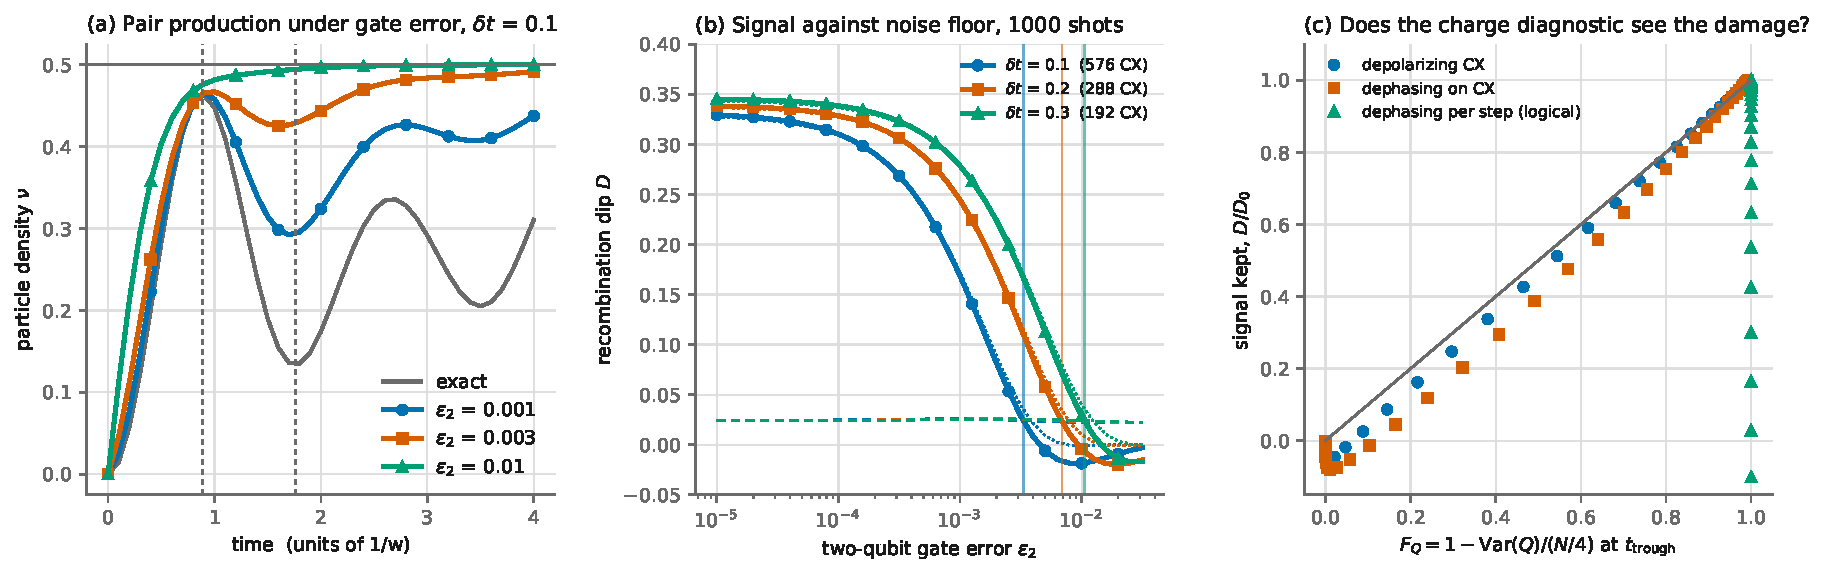
\includegraphics[width=\textwidth]{06_noise_threshold.pdf}
  \caption{(a) Particle density under depolarising gate error at
  $\delta t = 0.1$; dashed lines mark $t_{\mathrm{p}}$ and $t_{\mathrm{t}}$.
  (b) Recombination dip $D$ (solid), twice its shot-noise uncertainty at 1000
  shots (dashed), and the dip predicted from charge-conservation data taken at
  $\epsilon_0 \approx \epsilon^\ast/10$ (dotted). Vertical lines mark
  $\epsilon^\ast$. (c) Signal retained against the fidelity read from
  $\mathrm{Var}(Q)$, Eq.~\eqref{eq:FQ}; the diagonal is perfect prediction.
  Produced by \texttt{scripts/06\_noise\_threshold.py}.}
  \label{fig:threshold}
\end{figure}

\subsection{Does charge conservation predict the threshold?}

For gate noise it does, to within about 15\,\%, and it errs in one direction.
Using only the charge variance measured at one noise level
$\epsilon_0 \approx \epsilon^\ast/10$, the procedure of
Section~\ref{sec:budget-method} predicts thresholds 1.15, 1.14 and 1.17 times
the true value for $\delta t = 0.1$, $0.2$ and $0.3$ at 1000 shots, and 1.10 to
1.13 times it from $\epsilon_0 \approx \epsilon^\ast/3$. The prediction is always
optimistic: real gate noise erodes the dip somewhat faster than a global
depolarising channel with the same charge violation would.
Figure~\ref{fig:threshold}(c) shows why. The points for depolarising and for
gate-level dephasing noise lie close to the diagonal but slightly below it. At
$10^4$ shots the threshold sits at lower fidelity, where this small offset
matters more, and the overestimate grows to between 19 and 36\,\%.

For dephasing on the logical state the diagnostic fails completely.
$\mathrm{Var}(Q)$ stays at \num{1e-33} while the dip shrinks to zero at a
phase-flip probability of 0.036 per qubit per step, and the points in
Figure~\ref{fig:threshold}(c) form a vertical line at $F_Q = 1$. The CP
asymmetry is equally blind, because a uniform dephasing channel respects CP. A
charge-based diagnostic therefore bounds the damage from errors that move charge
and says nothing about errors that only scramble phases. This matters for the
literature: the error model Martinez \emph{et al.}\ fitted to their four-qubit
data was exactly this kind of dephasing~\cite{martinez2016}.
\todo{Discuss against Nguyen et al.\ symmetry protection, which targets coherent
errors, and Halimeh and Hauke on the slow growth of gauge violation.}

\subsection{The full budget and the optimal step size}

Figure~\ref{fig:budget}(a) puts all four sources together for one 1000-shot
measurement of $\nu(t_{\mathrm{t}})$ with 1\,\% readout error. Without gate
error the total error falls as $\delta t$ shrinks until it reaches the floor set
by shot noise and readout bias. With gate error it has a minimum. The optimal
step is $\delta t = 0.35$ (160 CX) at $\epsilon_2 = 3\times 10^{-4}$,
$0.44$ (128 CX) at $10^{-3}$, and $0.59$ (96 CX) at $3\times10^{-3}$: the worse
the hardware, the coarser the best Trotter step. At the optimum gate error
dominates, and the Trotter bias is between a quarter and two-fifths of it.
Refining the step past the optimum makes the answer worse, as the proposal
anticipated, and the figure shows by how much.

The decomposition depends on the observable (Figure~\ref{fig:budget}(b)). At
$\epsilon_2 = 10^{-3}$ and the optimal step, gate error is 89\,\% of the summed
squared error on the particle density, 59\,\% on the outer-link field, and only
29\,\% on the middle-link field, where Trotter error dominates. The middle-link
field is nearly immune to depolarising noise because its exact value at this
time, $-0.05$, is already close to its value in the maximally mixed state, zero;
the outer links sit at $-0.16$, far from their mixed-state value of $-0.5$. An
observable whose ideal value lies near its mixed-state value has little left for
depolarising noise to erase, and correspondingly little signal.

\begin{figure}[t]
  \centering
  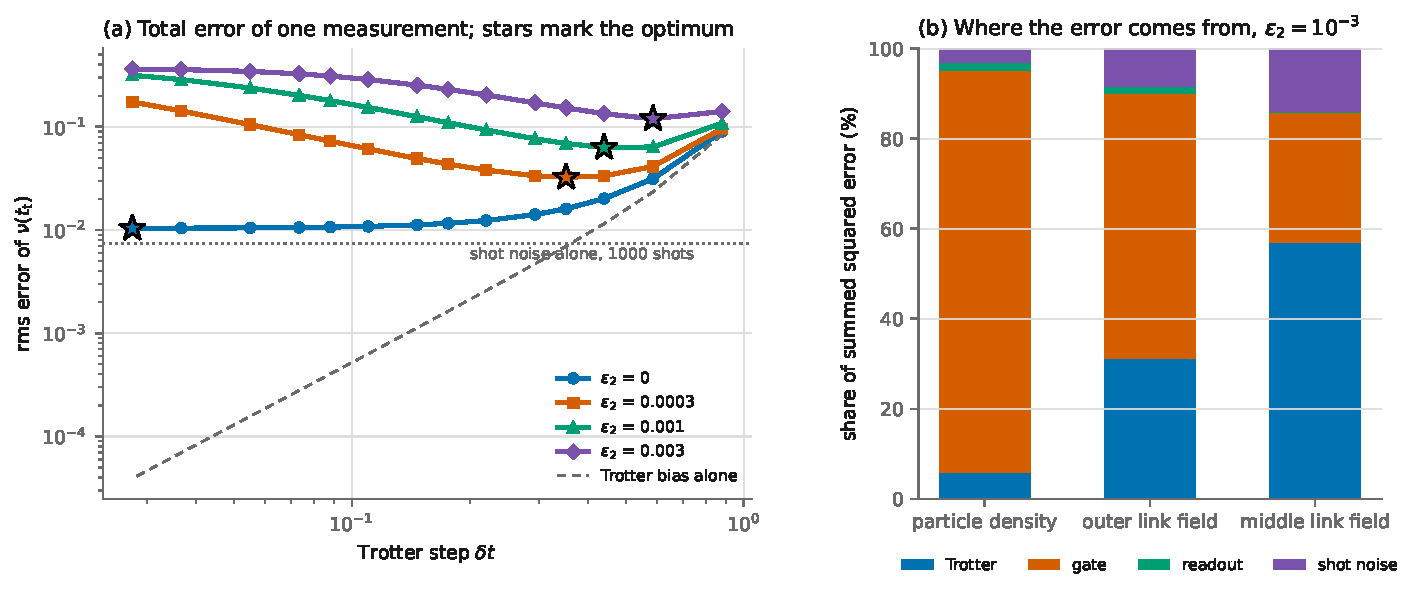
\includegraphics[width=\textwidth]{08_error_budget.pdf}
  \caption{(a) Root-mean-square error of a 1000-shot measurement of
  $\nu(t_{\mathrm{t}} = 1.76)$ against step size, with 1\,\% readout error, for
  four two-qubit error rates; stars mark the optimum. (b) Shares of the summed
  squared error at the optimum for $\epsilon_2 = 10^{-3}$. Produced by
  \texttt{scripts/08\_error\_budget.py}.}
  \label{fig:budget}
\end{figure}

\subsection{Ground state by SKQD}

At these parameters the ground state puts 71\,\% of its weight on the bare
vacuum $|0101\rangle$, 10\,\% on each of $|0110\rangle$ and $|1001\rangle$,
7.5\,\% on $|0011\rangle$, 1.7\,\% on $|1010\rangle$, and \num{6.5e-4} on
$|1100\rangle$, the configuration with the longest flux string. Confinement
suppresses exactly the bitstrings SKQD is most likely to miss.
Figure~\ref{fig:skqd} shows the exact expected SKQD energy error against the
number of shots per Krylov step. With four full Trotter steps of
$\delta t = 0.3$, the relative energy error falls below $10^{-3}$ at 12 shots
per step and below $10^{-6}$ at about 100. With a single hopping-only step, as
in Rosanowski \emph{et al.}, 50 shots are needed for $10^{-3}$. Gate error at
$\epsilon_2 = 3\times10^{-3}$ makes SKQD slightly worse, not better: 20 shots per
step instead of 12. Noise spreads probability over all sixteen bitstrings, but
the ten charged ones are discarded, so at a fixed shot count fewer samples land
in the neutral sector. At $N = 4$ the only error left in SKQD is coverage, and a
few hundred shots remove it.

\begin{figure}[t]
  \centering
  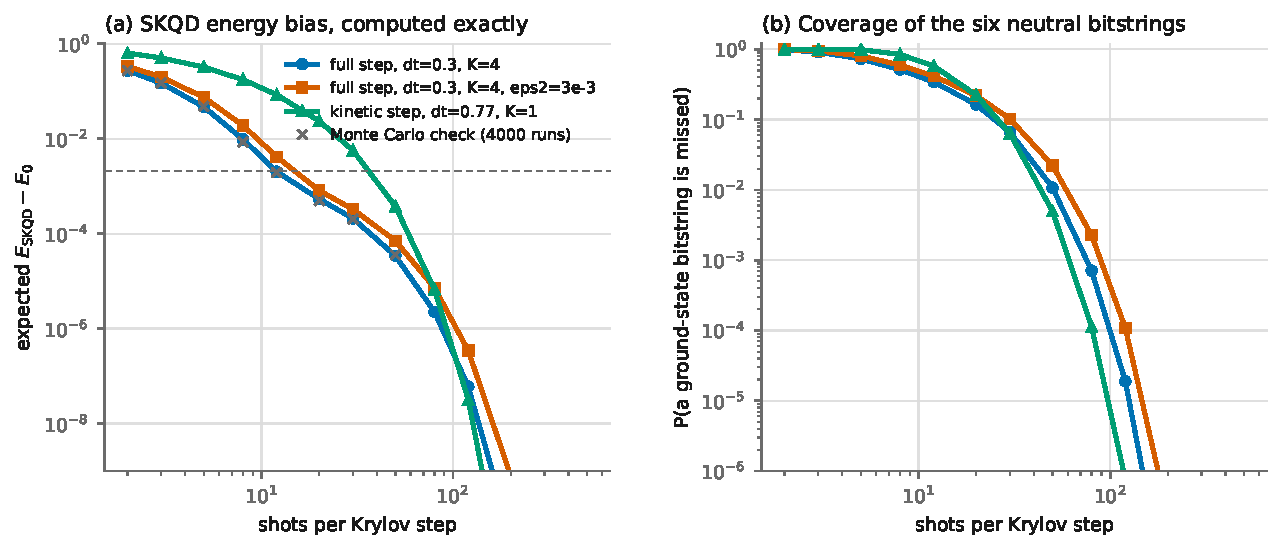
\includegraphics[width=0.9\textwidth]{07_skqd.pdf}
  \caption{(a) Exact expected SKQD energy error against shots per Krylov step,
  for four full second-order steps without and with gate error, and for one
  hopping-only step; crosses are a Monte Carlo check. The dashed line is a
  relative error of $10^{-3}$. (b) Probability that at least one bitstring of the
  ground state is never sampled. The single-step configuration uses a quarter of
  the total shots at the same horizontal position. Produced by
  \texttt{scripts/07\_skqd\_ground\_state.py}.}
  \label{fig:skqd}
\end{figure}

% ============================================================================
\section{Discussion}
\label{sec:discussion}
% ============================================================================

\todo{Due with the Results and Discussion draft. Three paragraphs planned:
(1) the depth rule $\epsilon^\ast n_{\mathrm{CX}} \approx 2$ against published
gate counts (Martinez: more than 200 gates; Farrell: 13,858 two-qubit gates) and
fidelities; (2) what the optimistic bias and the dephasing blind spot mean for
symmetry-based diagnostics in the literature (Martinez leakage, Nguyen symmetry
protection, Halimeh and Hauke); (3) limitations: depolarising and dephasing
models only, no coherent or correlated error, no amplitude damping, one
parameter point, $N = 4$, and a coarse lattice far from the continuum.}

% ============================================================================
\section{Discussion}
\label{sec:discussion}
% ============================================================================
% FIRST DRAFT. Every number from this project is printed by scripts 04-08
% (VERIFICATION.txt). Every statement about a paper was checked against the
% paper. Derived numbers: 247 and 181 CX acting on the average qubit are twice
% Farrell et al.'s CNOT counts (13,858 and 10,154) over 112 qubits; their Table
% III caption prints the same numbers as "twice the number of CNOTs/qubit",
% because they count each CNOT once per circuit, not once per qubit it touches;
% 288 per qubit is 2 x 576 / 4; Shaw et al.'s worst-case CX error is the
% non-identity Pauli probability of the depolarising channel, 15/16 x 4/3 eps2
% = 1.25 eps2, so their bound fails at eps2 n_CX = 0.5 / 1.25 = 0.4.

\subsection{The depth rule and published experiments}

Each of the four qubits takes part in $n_{\mathrm{CX}}/2$ CX gates on average,
so the 1000-shot rule $\epsilon^\ast n_{\mathrm{CX}} \approx 2$ also reads per
qubit: without mitigation the signal is lost once the summed infidelity of the
gates on the average qubit reaches about one.

The per-qubit form is the one to carry to larger devices, since Farrell
\emph{et al.}\ argue that two-qubit gates per qubit, not their total, limit
large simulations~\cite{farrell2024}. Their deepest hadron circuit has
\num{13858} CX gates on 112 qubits, so 247 act on the average
qubit~\cite{farrell2024b}, close to the 288 of the $\delta t = 0.1$ trough
circuit here. With 181 on the average qubit their data showed no wave packet
until heavy error mitigation restored it, and the results still often differed from classical
simulations by many standard deviations~\cite{farrell2024b}. Neither Farrell
paper quotes its device's gate error, and Martinez \emph{et al.}\ give no gate
fidelity and use no CX gates~\cite{martinez2016}, so none of the three can test
the rule. Rosanowski \emph{et al.}\ quote a typical two-qubit fidelity of
99.6(2)\,\% for their trapped-ion processor~\cite{rosanowski2025}; its error,
$2\times10^{-3}$ to $6\times10^{-3}$, straddles $\epsilon^\ast$ at
$\delta t = 0.1$ and lies below it at 0.2 and 0.3.

Shaw \emph{et al.}\ bound the gate-error bias by the number of noisy CX gates
times their worst-case error, $1.25\,\epsilon_2$ for depolarising
CX~\cite{shaw2020}. On the positron density, which cannot exceed $\tfrac12$,
the bound says nothing beyond $\epsilon_2 n_{\mathrm{CX}} = 0.4$, a fifth of
where the dip here is lost: the small-scale comparison the authors ask for,
though their lattice keeps the gauge field.

\subsection{The optimal step}

Knee and Munro~\cite{knee2015} and Shaw \emph{et al.}~\cite{shaw2020} predict
that the best Trotter step grows with the gate error, and the optima here agree:
five, four and three steps to $t_{\mathrm{t}}$ for $\epsilon_2 =
3\times10^{-4}$, $10^{-3}$ and $3\times10^{-3}$, too few integer points to test
a power law. Experiments have made the same choice by eye: Klco \emph{et al.}\
moved from $\delta t = 0.1$ to $0.25$ and Nguyen \emph{et al.}\ doubled their
step, each because after a few steps hardware error, not Trotter error,
dominated~\cite{klco2018,nguyen2022}. At $\epsilon_2 = 3\times10^{-4}$ the
optimal step, 0.35, sits at the 1000-shot crossover at $t_{\mathrm{t}}$, 0.36;
at larger error it is coarser, so at the best achievable step the Trotter error
exceeds the shot noise.

\subsection{What a symmetry check can and cannot tell}

Martinez \emph{et al.}\ called the leakage out of the neutral states a useful
measure of fidelity, and Nguyen \emph{et al.}\ reported it, but neither turned a
charge violation into an error on an observable~\cite{martinez2016,nguyen2022}.
Section~\ref{sec:results} does.

The prediction is optimistic because Eq.~\eqref{eq:FQ} assumes a global
depolarising channel, as do the rescaling methods of Vovrosh \emph{et al.}\ and
Urbanek \emph{et al.}, who treat it as an approximation for deep circuits on
many qubits~\cite{vovrosh2021,urbanek2021}. Four qubits are far from that
regime, and the optimistic bias is the residual: local noise erodes the dip
faster than a global channel with the same charge violation. Farrell \emph{et
al.}\ replaced a rescaling that assumes every qubit decoheres at the same rate
by one factor per observable~\cite{farrell2024}, and still attribute part of
their disagreement with simulation to the simplicity of the assumed
noise~\cite{farrell2024b}. Since every prediction from unsampled
data overshot the true threshold, a threshold read from a symmetry check is best
treated as an upper bound on the usable depth, though the prediction from a
single 1000-shot run falls below the true threshold 8 to 20\,\% of the time.

The blind spot is general, since a symmetry check cannot catch an error that
commutes with the symmetry~\cite{cai2023}, and the noise model of the first
experiment falls in it. Martinez \emph{et al.}\ fitted a phase-flip probability
per qubit per step to their postselected data, choosing that model because
postselection already partly corrects population errors~\cite{martinez2016}.
Their leakage of 14 to 31\,\% and their fitted dephasing thus describe
complementary parts of the noise, and $\mathrm{Var}(Q)$ would read exactly zero
for the second.

\subsection{The ground state}

Rosanowski \emph{et al.}\ argue that SKQD resists noise because only which
bitstrings are sampled matters, provided every needed one appears at least
once~\cite{rosanowski2025}. The exact calculation confirms it: gate error at
$\epsilon_2 = 3\times10^{-3}$ costs only 15 shots per step instead of 12. The
neutral sector grows as $\binom{N}{N/2}$, so rare bitstrings left
unsampled~\cite{miura2026} will limit larger lattices.

\subsection{Limitations}
\label{sec:limitations}

The noise models are the main limitation. Depolarising and dephasing noise act
on each gate independently and without memory; real devices also have coherent
errors such as over-rotation, which could shift or imitate the dip, correlated
errors, and amplitude damping, whose end state Eq.~\eqref{eq:FQ} reads as
perfect fidelity (Section~\ref{sec:noise}). Farrell \emph{et al.}\ saw
systematic errors that grow with the rotation angle of the
gates~\cite{farrell2024b}, which no depolarising model produces and which would
favour smaller steps. Readout error is left out of the threshold; all qubit
pairs are coupled, whereas nearest-neighbour hardware needs SWAP gates for the
RZZ between sites 1 and 3; and the criterion $D \le 2\sigma_D$ is a choice.
Everything is at one parameter point on four sites (twelve for the classical
check of Figure~\ref{fig:sizes}), a coarse lattice far from the continuum, in
simulation with assumed noise.

% ============================================================================
\section{Conclusion}
\label{sec:conclusion}
% ============================================================================

The four-site lattice Schwinger model was simulated with Trotter error, shot
noise, gate error and readout error separated, every stage checked against
exact diagonalisation, and the published curves of Martinez \emph{et al.}\
reproduced. At 1000 shots the Trotter error on the particle density falls
below the shot noise at a step of 0.18 at $t = 3$. At the same shot count the
pair-production signal is lost when the two-qubit infidelity times the CX count
of the deepest circuit reaches about two, at all three step sizes tried, and the
best step grows with the gate error. The charge variance predicts that threshold
with an optimistic bias of 10 to 17\,\% for depolarising noise and a larger one
for dephasing on the gates, and misses it entirely for dephasing between time
steps, the model fitted to the first experiment on this system. Whether these
numbers survive coherent and correlated errors, and real hardware, is the next
question.
  % Discussion and Conclusion

\section*{Statement on AI assistance}

I used AI tools to write the scaffolding of the code, to debug it
(particularly the sign conventions in the Jordan--Wigner strings), to find my
way through the literature and to draft text. The derivations, the design of
the numerical experiments and the analysis are mine. Every claim an AI tool
made about a paper was checked against that paper.

The checks built into the project caught errors in what the tools drafted, all
corrected in this version. Two were in the code: a wrong guess about Qiskit's
qubit order and an ill-conditioned step in the Ising-chain check. The third was
a physics claim, that dephasing on the compiled gates is invisible to the
charge diagnostic. Simulation showed this holds only for dephasing on the
logical state (Section~\ref{sec:diagnostics}).

A review of the draft then found statements that the numbers contradicted. Two
test tolerances were quoted as measured residuals. The symmetry argument for
Eq.~\eqref{eq:cp} claimed more than it proved, and the two components of $\psi$
were described wrongly. The Hellmann--Feynman check was presented as stronger
than it is, and the account of where the energy of the produced pairs comes
from had it backwards.

Checking every literature claim against its paper, before the Discussion was
written, found four errors in the Introduction and Methods. Shaw \emph{et al.}'s
bound adds the Trotter and gate biases linearly, not in quadrature. Rosanowski
\emph{et al.}\ report energies on up to 20 qubits, not 30, and quote their gate
fidelity rather than measure it. Halimeh and Hauke's penalty result had been
quoted without its restriction to coherent errors. Reproducing the curves of
Martinez \emph{et al.}\ found the last one: Methods had written the first-order
step in reverse order.

\clearpage
\bibliographystyle{apsrev4-2}
\bibliography{refs}

\end{document}
